\documentclass[a4paper,11pt,oneside]{book}


\newcommand{\doctitle}{\begin{spacing}{2}
		MSc Thesis Report\\ 
		\begin{Huge}
			Manoeuvrability and communication requirements for safe operation of autonomous and unmanned vessels
		\end{Huge}
	\end{spacing}}

\newcommand{\docauthor}{Ingmar Wever (4161041)}

\usepackage{acronym}
\usepackage{afterpage}
\usepackage[noend]{algpseudocode}
\usepackage{appendix}
\usepackage{booktabs} % improving tables
\usepackage{enumitem}
\usepackage{epigraph}
\usepackage{include/epipart}
\usepackage{float}
\usepackage[margin = 1.2in]{geometry} % change the page margins
\usepackage{textcomp} % To avoid warnings in gensymb
\usepackage{gensymb} % for generic symbols
\usepackage{graphicx} % to use \includegraphics
\usepackage{hyperref} % adding urls using \url
\usepackage[utf8]{inputenc} % makes sure other characters than ASCII can be used
\usepackage{listings} % to add code snippets
\usepackage{multicol} % use multiple columns in text
\usepackage{parskip} % makes sure that a line is skipped after every paragraph
\usepackage{pifont} % For checkmark and cross mark
\usepackage{setspace} % set spacing in paragrahs like contents
\usepackage{subcaption} % for caption of subfigures
\usepackage{tikz} % for graphics, also build front cover using tikz
\usepackage{titlesec, color}
\usepackage[textsize=footnotesize]{todonotes} % placing todo notes and summarizing them at start of document
\usepackage{wrapfig}

%% Todonots setting
\presetkeys{todonotes}{inline, bordercolor=orange, backgroundcolor=blue!10, linecolor=black}{}

%% Bibliography style
\bibliographystyle{include/tudelft-report}

%% Change font to sans-serif
\renewcommand{\familydefault}{\sfdefault}

%% Folder with figures
\graphicspath{{figure/}}

%% Epigraph size
\setlength{\epigraphwidth}{0.45\textwidth}

%% No line-breaking
\hyphenpenalty=10000

%% Captions always centered
\captionsetup{justification=centering}

%% Symbols to link dependent variables
\newcommand{\performance}{$\clubsuit$}
\newcommand{\trust}{$\diamondsuit$}
\newcommand{\participant}{$\odot$}
\newcommand{\SA}{$\spadesuit$}
\newcommand{\satisfaction}{$\heartsuit$}
\newcommand{\protocol}{$\star$}

%% Text lay-out
% Customize chapter style
\titleformat
{\chapter} % command
[hang] % shape
{\bfseries \LARGE \raggedright} % format
{\thechapter \hspace{5pt} \textcolor{cyan} {$|$} } % label
{0pt}
{\bfseries \LARGE \raggedright} % before-code
[] % after-code

\titlespacing
{\chapter}
{30pt} % Left
{-30pt} % Top
{5pt} % Bottom
%%  Hyperlink colors
\hypersetup{ %setup hyperlinks
    colorlinks,
    citecolor=black,
    filecolor=black,
    linkcolor=black,
    urlcolor=black
}

\setlength{\parindent}{0pt}

%% Line spacing
\renewcommand{\baselinestretch}{1.35} 

%% Tikz settings
\usetikzlibrary{arrows,shapes,positioning,shadows,trees}


%% Front cover, blank page, title page command
\newcommand{\emptyDoublePage}{
	\newpage
	\phantom{-}
	\newpage
}

\newcommand{\addCoverPage}{
	%% Create an empty page for cover.
	\clearpage
	\thispagestyle{empty}

 	%% Building cover
	\begin{tikzpicture}[remember picture,overlay]
		\node (picture) at (current page.center)
		{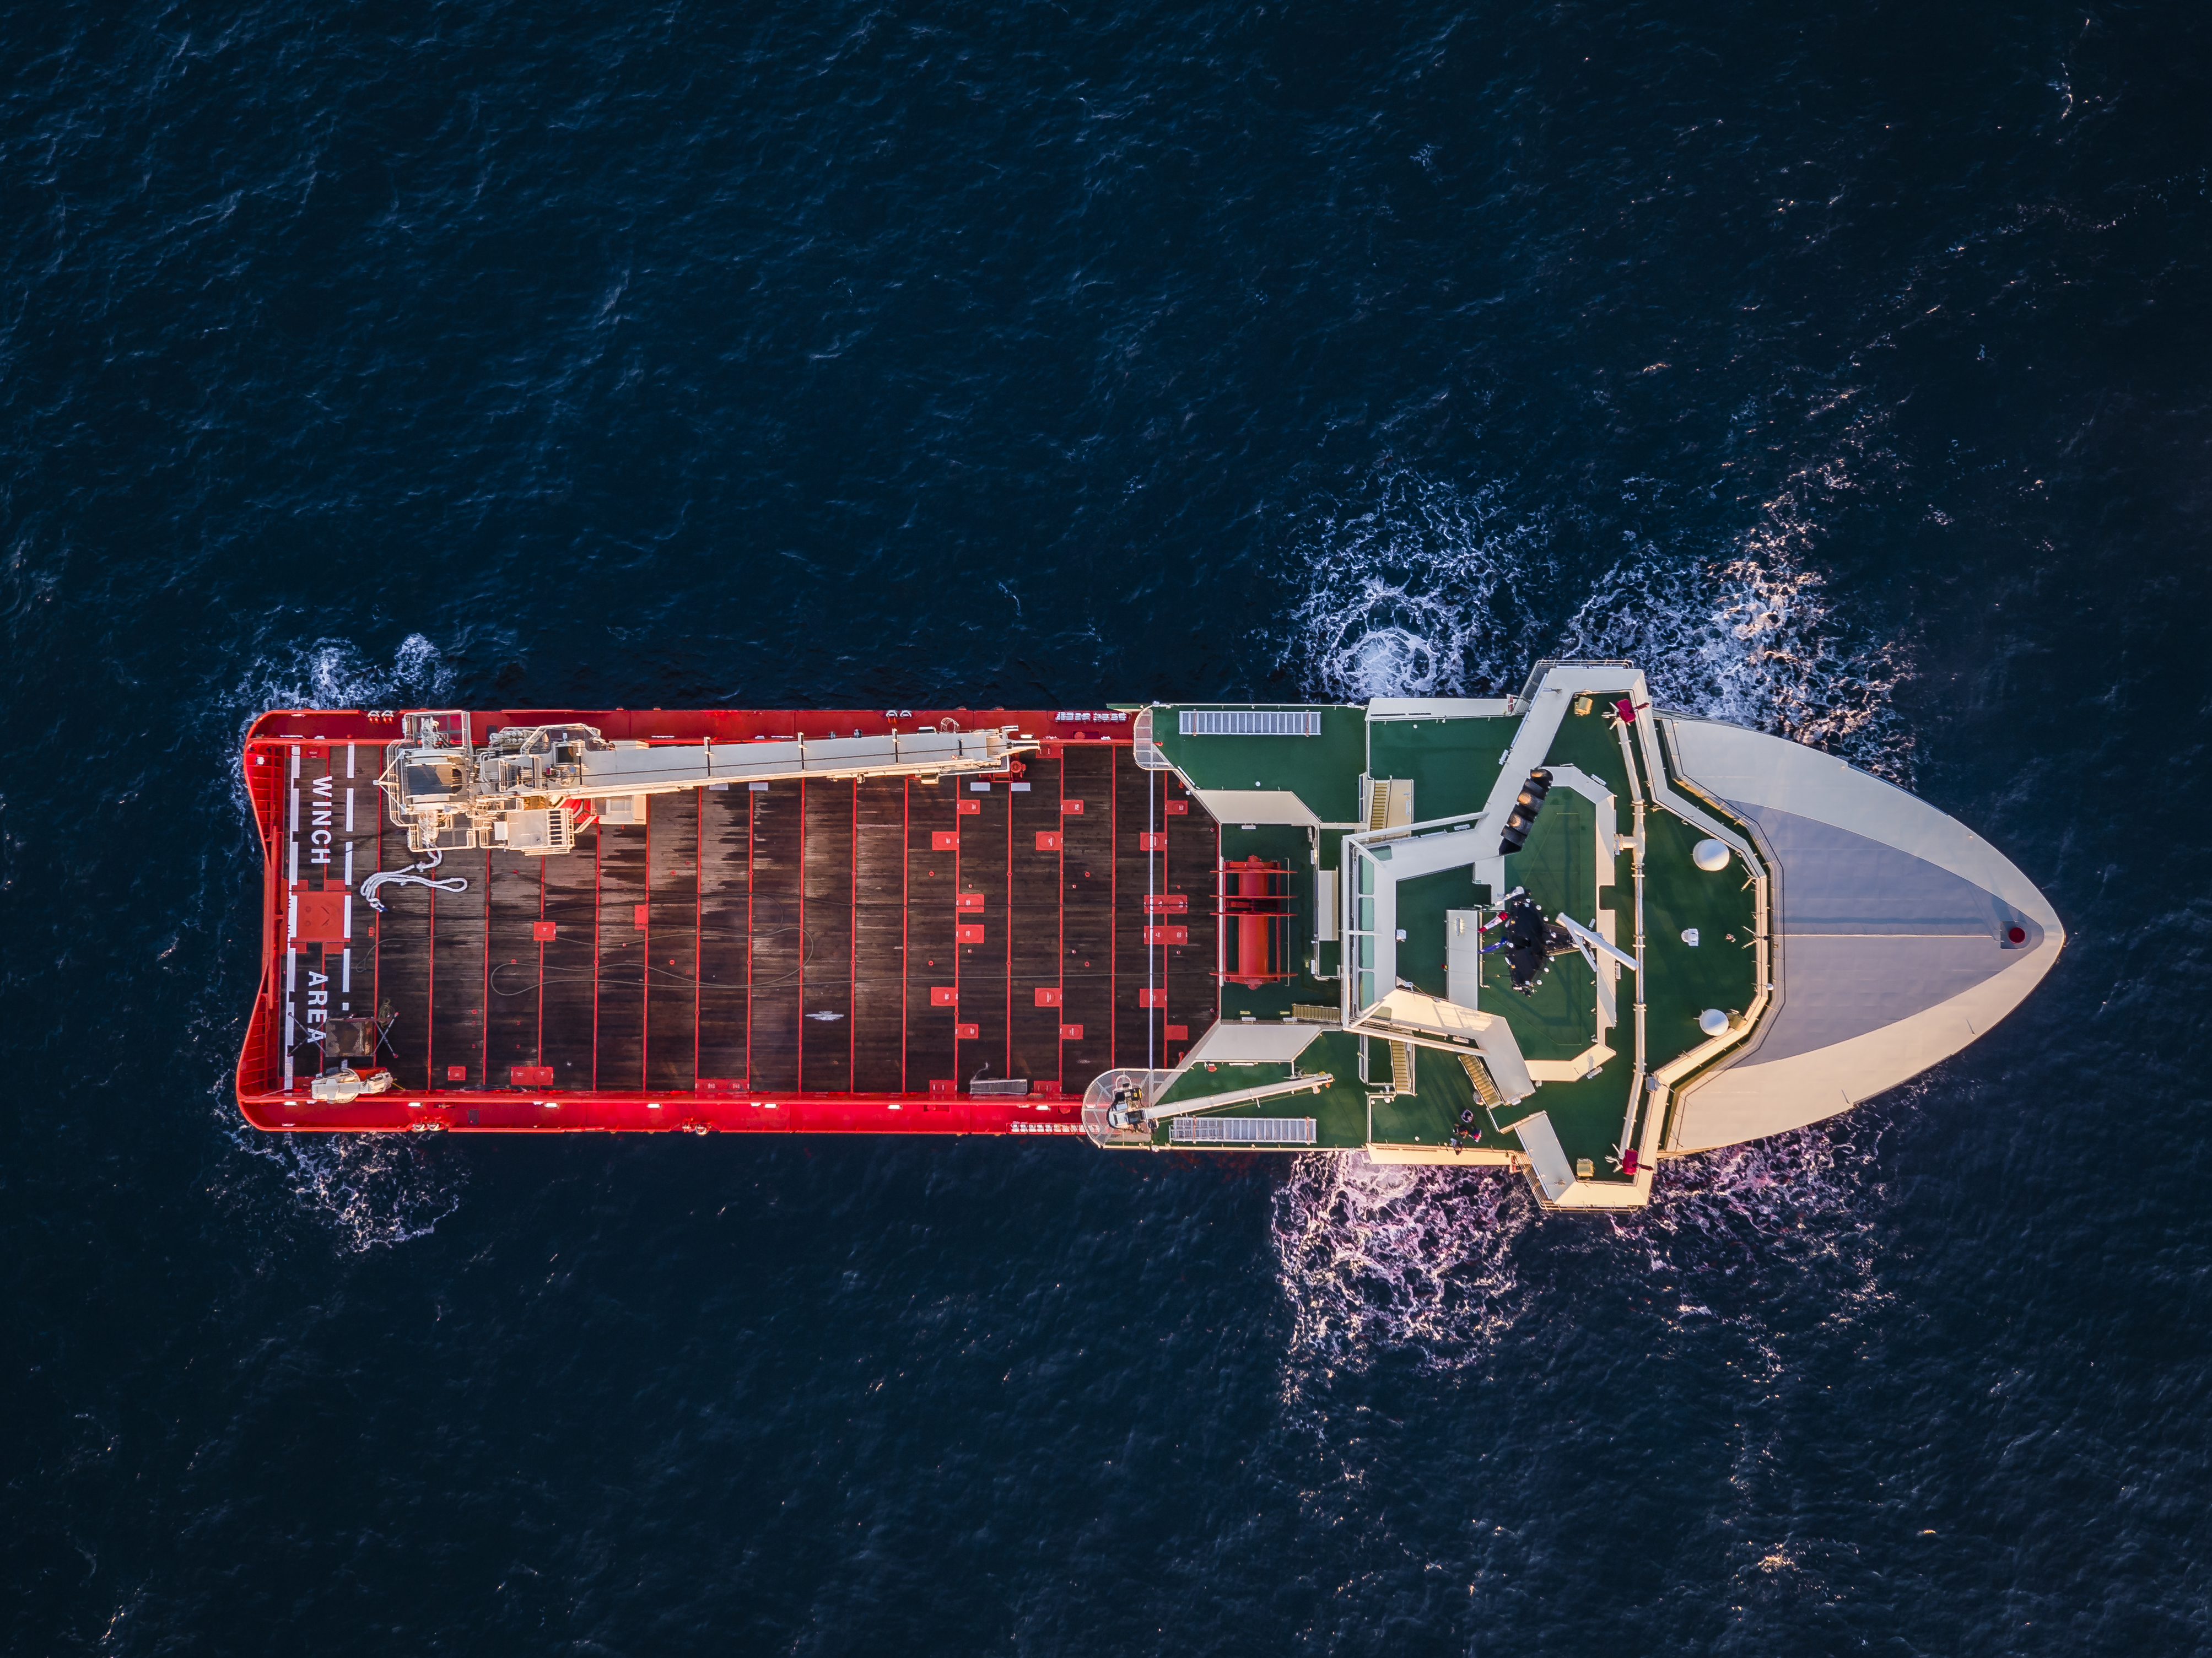
\includegraphics[height=\paperheight, keepaspectratio]{cover_PSV_5000_top.jpg}};
		
		\node (white-glow) at (current page.center) [fill = white, minimum width = \paperwidth, minimum height = \paperheight, opacity = 0.15]{};
		
		\node (title-box-bg) at (current page.east) [fill = gray, minimum width=.5\paperwidth, minimum height=7cm, fill opacity = 0.85, xshift=-.3\paperwidth, yshift=-5cm, text=white] {};
		
		\node (title-box) at (current page.east) [minimum width=.5\paperwidth, minimum height=7cm, align=left, xshift=-.3\paperwidth, yshift=-5cm, text=white] {
			\hspace{.5cm}
			\huge{MSc Thesis Report} \\ \\
			\Large{Manoeuvrability and communication} \\
			\Large{requirements for safe operation when} \\
			\Large{manned and unmanned vessels meet} \\ \\
			Ingmar Wever \\
			\today
			
		};
	
		\node (black-bar) [fill = black, minimum width=.5\paperwidth, minimum height=0.2cm, yshift = -3.4cm, fill opacity = 0.7] at (title-box){};
		
		\node (cyan-bar) [fill = cyan, minimum width=.5\paperwidth, minimum height=0.2cm, yshift = -3.6cm, fill opacity = 0.7] at (title-box){};
		
		\node (white-bar) [fill = white, minimum width=.5\paperwidth, minimum height=1.5cm, yshift = -4.5cm, fill opacity = 0.95] at (title-box){
		
			\includegraphics[height=1.3cm, keepaspectratio]{TU_Delft_logo_RGB.png}
			\hspace{.8cm}
			\includegraphics[height=.8cm, keepaspectratio]{Damen_logo.png}
		};
	
		
	\end{tikzpicture}
}

\newcommand{\addEmptyPage}{
	%% Create empty page for two-sided printing
	\clearpage
	\setcounter{page}{0}
	\thispagestyle{empty}
	\vspace*{6cm}
	\begin{center}
		This page is intentionally left blank.
		
		\tiny{(Except for the above line.)}

	\end{center}
	\todo{Titels begeleiders and graduation date}
}

\newcommand{\addTitlePage}{
	\begin{titlepage}
	
	%% Title page
	\newpage
	
	\centering
	\Large
	\vspace*{1cm}
	Thesis Report for the degree of \\ 
	MSc Marine Technology and MSc Computer Science\\
	\vspace{1cm}
	\begin{spacing}{2}
		\begin{Huge}
			Manoeuvrability and communication requirements for safe operation when manned and unmanned vessels meet
		\end{Huge}
	\end{spacing}
	\large
	\vspace{1cm}	
	by Ingmar Wever
	at Damen Shipyards and TU Delft
	
	\today
	
	\vspace{1.5cm}
	\footnotesize
	This thesis (SDPO.18.048.m) is classified as confidential in accordancewith the general conditions for projects performed by the TU Delft. 
	
	\vspace{3cm}
	\normalsize
	\begin{tabular}{lll}
		Student: & Ingmar Wever & 4161041 \\
		Project duration: & \multicolumn{2}{l}{September 2017 -- November 2018} \\
		& & \\
		Supervisors: & Dr.ir. Robert Hekkenberg & TU Delft, Ship Design \\
		& Prof.Dr. Mark Neerincx & TU Delft, Interactive Intelligence \\
		& Toine Cleophas & Damen Shipyards, R\&D \\
		Committee members: & Peter de Vos MSc. & TU Delft, Marine Engineering \\
		& Dr.ir. Willem-Paul Brinkman & TU Delft, Interactive Intelligence \\
	\end{tabular}

	\end{titlepage}
}
	

\begin{document}
\frontmatter

\makeCover % Cover, blank page and title page

\listoftodos[Notes]
\clearpage

\chapter{Preface}
I did start my journey to become a shipbuilder in 2011. Delft has become my second home in the years since. In those years I have not only been introduced in the world of shipbuilding. But I have also developed myself towards a "Delftse Ingenieur". This report is the last step in this journey. And although the writing of this report has been an individual accomplishment. I could not have done it without the help of some very talented, critical, caring and enthusiastic people around me.

First of all, I would like to thank all the people I have met at Damen Shipyards, where the doors were always open to ask questions and discuss our extraordinary industry. A special thanks to Toine Cleophas, my supervisor at Damen. Besides being a supervisor, he has also been my mentor. He showed me the maritime industry and Damen from his perspective, which I could not have learned at any university. Thank you for the late afternoon discussions at the office, in the car, and with a beer in our hand.

Furthermore, I would like to thank Robert Hekkenberg as a guide in the world of academics. By questioning the steps I took and guiding the scope. He has helped me through many iterations, which have resulted in not only a good design, but also a design well sold.

Another thank you goes to Mark Neerincx, as supervisor, he has helped me to explore the world of human-computer interaction research. With his academic knowledge and practical experience did he help me to keep the balance between developing knowledge and a product.

Beside my supervisors have there been many more people involved in the steps taken, which resulted in this thesis. It is not possible to name all of you.
I want and need to show my utmost gratitude to some exceptional people. My parents, pappa and mamma, I want to thank you for giving me the roots to get back to, and wings to fly beyond the horizon.\\


\begin{flushright}
	\textit{Ingmar Wever\\
		Amsterdam, December 2018}
\end{flushright}
\chapter{Abstract}
\todo{Schrijf samenvatting}

\begin{spacing}{1}
	\listoffigures
\newpage
\listoftables
\todo{list of used symbols?}
\newpage

\chapter*{List of Abbreviations}
\begin{acronym} % Give the longest label here so that the list is nicely aligned
	\acro{AIS}{Automatic Identification System}
	\acro{AMS}{Alarm Management System}
	\acro{ARPA}{Automatic Radar Plotting Aid}
	\acro{BNWAS}{Bridge Navigational Watch Alarm System}
	\acro{CAM-HMI}{Central Alert Management - Human Machine Interface for presenting and handling of alerts}
	\acro{COLREGs}{Convention on the International Regulations for Preventing Collisions at Sea}
	\acro{CPA}{closest point of approach}
	\acro{ECDIS}{Electronic Chart Display Information System}
	\acro{ENC}{Electronic Navigational Chart}
	\acro{GNSS}{Global Navigation Satellite System}
	\acro{GPS}{Global Positioning System}
	\acro{IEC}{International Electrotechnical Commission}
	\acro{IHO}{International Hydrographic Organization}
	\acro{IMO}{International Maritime Organization}
	\acro{Navtex}{Navigational text Messages}
	\acro{no-UI}{Non-visual User Interface}
	\acro{OoW}{Officer of Watch}
	\acro{sCE}{situated Cognitive Engineering}
	\acro{SMCP}{Standard Maritime Communication Phrases}
	\acro{SMNV}{Standard Marine Navigational Vocabulary}
	\acro{SOLAS}{International Convention for the Safety of Life at Sea}
	\acro{STCW}{International Convention on Standards of Training, Certification and Watchkeeping for Seafarers}
	\acro{TEU}{Twenty foot Equivalent Unit}
	\acro{UID}{User Input Device}
	\acro{VDES}{VHF Data Exchange System}
	\acro{VHF}{Very High Frequency radio}
\end{acronym}
	
	\clearpage
	\setcounter{tocdepth}{1}
	
	\tableofcontents
\end{spacing}
\clearpage

\mainmatter

\chapter*{Introduction}
\label{sec:introduction}
\addcontentsline{toc}{chapter}{Introduction}

The Maritime industry is tapping into the world of automation and digitalisation. The automation level of vessels is proliferating. Vessels are getting connected to the shore by different means. Operational data is becoming available and enriched with other data sets like design data, weather data and maintenance data. These technologies boost the development of autonomous and unmanned vessel designs \cite{Blanke2017}. 
At the same time is the Maritime Industry facing challenges when it comes to crewing and safety \cite{Cappelle2018}. Combined with an increasing competition it is hard to make healthy margins. These trends trigger Maritime Industry to embrace autonomous sailing technologies to secure a healthy future. These business developments reflect in the significant amount of research and development projects \cite{SMASH2017} \cite{Eriksen2017} \cite{MUNIN2016} \cite{Sames2017} \cite{RollsRoyce2015} \cite{Waterborne2016}. Each one of these projects tackles one or more challenges in the development of autonomous sailing. However, is the challenge of communication between unmanned and manned vessels not been tackled \cite{Saarni2018}. In chapter~\ref{ch:future}, these challenges and related projects are discussed. Currently, no solutions are available. However, this is necessary to ensure the safety of all vessels: manned, unmanned, remote, automated and autonomous.

This report presents the results of the research on communication between unmanned autonomous sailing vessels and manned vessels. It gives a design philosophy which has been translated in a methodology for handling communication which is eventually turned into protocols which are derived based on theory and validated through simulations.

% More people start to believe in the possibilities of unmanned and autonomous shipping, as there are many projects which try to develop the necessary technologies \cite{SMASH2017} \cite{Eriksen2017} \cite{MUNIN2016} \cite{Sames2017} \cite{RollsRoyce2015} \cite{Waterborne2016}. The major reason for the development of autonomous ships are the benefits for operational expenses. But one of the major reasons for acceptance is the mitigation of human errors. Which can be achieved by taking out humans from the chain of command. This will, however, introduce new challenges \cite{Saarni2018}. In chapter \ref{ch:future} these challenges and corresponding projects are discussed. One of the less explored challenges is the issue of communication. This becomes harder between manned and unmanned vessels. Communication is used to share information on the intentions or discuss future actions. At the moment there is no protocol which can be used by unmanned vessels. However this is necessary to ensure the safety of all vessels: manned, unmanned, remote, automated and autonomous.
% To solve this challenge, there are two possibilities: Avoid the need for communication, or develop a new communication protocol.

\subsubsection*{Context}
In many situations is the \acf{COLREGs} sufficient to determine the intentions of other vessels \cite{IMO1972}. They can be seen as ship separation rules, which guide all vessels to make early and correct alterations to their course. It will take more time to assess the situation when using \ac{VHF}. Meaning there is less time to act, which limits the possible strategies. These rules do also apply to autonomous ships, and thus can be used when manned and unmanned vessels meet.
Examples are to stay on the starboard side of the shipping lane, and not to cross other ships with a small relative angle. When this does not happen, communication is necessary. When this communication doesn't occur correctly, there is a much higher risk of accidents (appendix \ref{app:accidents}). Thereby are there also situations in which regulations are contradictory, such as the accident between Artadi and St-Germain as described in appendix \ref{sec:artadiVSst-germain}. These contradictions occur more often in complex situations, such as a harbour approach.

The risks when \ac{COLREGs} are not sufficient can be mitigated by taking decisions, well in advance. What well in advance means, depends on the manoeuvrability and operation of a vessel. A cargo vessel will follow common paths, while a small tugboat might move around much more. These situations result in more false positives on potential collisions with other vessels, when using the same safety domain and evaluation system. The impact of manoeuvrability means that it is necessary to think ahead several minutes with a large ship, while this is much shorter for a small tugboat. This time-domain for decision making depends not only on the ship characteristics but also on the waterway characteristics. Chapter~\ref{ch:model} discusses this in more detail. Examples are the depth, traffic separation schemes and harbour entrances.

If it is not possible to take decision well in advance, it is often due to a lack of information. Communication solves this problem. This communication between manned vessels happens in different ways. Most important is communication via \ac{VHF}, thereby is information from the AIS used to identify ships. Also can this information help to determine the intentions of the vessel, based on the type of vessel or destination. The used protocols for these systems are discussed in appendix~\ref{app:systems}

\subsubsection*{Design philosophy}
We developed a strategy to cope with the challenge of communication between manned and unmanned vessels, without introducing new systems to the bridge of manned vessels. 
First, we will try to avoid the need for communication, by staying well clear from other ships. When this is not possible, there is a need for communication. A new protocol must be developed for this communication.
This strategy can be used as a foundation to build a system for decision making which ensures safe operation of both manned and unmanned vessels. Different steps must be taken to implement this strategy. 

First insights have been acquired on the decision model for safe navigation, to determine which factors are taken into account to make a decision. The next step is to learn how these factors influence the decision process. This can also be used to determine the critical situations. Showing when it isn't possible to navigate without communicating. Leaving some specific situations for which a communication protocol must is necessary. Using the \acf{sCE} method, the operational demands, relevant human factors and envisioned protocol could be defined. The current state of the maritime industry is taken into account.

\subsubsection*{Research questions}
The report will touch upon different research domains in more detail: Maritime Technology and Computer Science. The part on maritime technology focuses on the situation where manoeuvring is just enough. While the computer science part will focus on the development of the communication protocol. Answering the following research questions:

\begin{quotation}
	\emph{How do ship manoeuvrability characteristics influence the domain for decision making, to ensure that the chosen strategy will result in a passing distance which does not require communication?} 
\end{quotation}

\begin{quotation}
	\emph{Will a protocol based on existing maritime systems and communication protocols be sufficient to ensure safe navigation, while manned and unmanned vessels encounter each other?}
\end{quotation}

\subsubsection*{Report structure}
This research has three parts. In those parts, the challenge of communication between manned and unmanned vessels is considered. Part~\ref{part:general} gives a more detailed context of autonomous shipping. This context is used with a decision-model to show why communication is a challenge, and how this challenge can be tackled.

Part~\ref{part:MT} aims to determine how communication can be avoided. To resolve this, it is important first to determine when communication is necessary, which is in case of critical situations. These situations are tested in a simulation environment. The time-domain for decision making can be determined to ensure safe operation in these simulations. These situations are simulated, using a validated manoeuvring model. Thereby is evaluated that ships need communication in fewer cases if the decision-domain is improved.

Part \ref{part:CS} will focus on critical situations where communication is a must. Currently, a communication protocol between manned and unmanned vessels has not been part of any known project. Communication is necessary in cases where there is a lack of trust, missing information or the time-domain for decision making becomes critical. To ensure a fest implementation of the communication protocol between manned and unmanned vessels, will it be based on existing systems and protocols. The aim of this part is to validate if it is possible to define a protocol using the \acf{sCE} method, which will be accepted by seafarers.


\part{The problem of communication for autonomous vessels}
Safety at sea has been a relevant topic as long as ships exist. There are several factors which have a big influence on safety. First and foremost is communication in all the ways where information is shared. Before the invention of radio communication, ships literally lost all connection with the shore and other ships when setting sail. Flags were used when ships were close to others ships or to the shore. This form of communication was not complete as it only gave limited insight in the intentions of other vessels for example.

New technologies lead to new ways for communication, which subsequently lead to a safer industry. But new technologies also lead to complexer situations. As ships get bigger and perform more complex operations, resulting in less manoeuvrability. In those situations it is very important to share the right information. The current situation of the maritime is assessed together with a summary of likely new technologies related to navigational safety. 

To give insight in the current situation of the shipping industry, first some accidents are discussed and which lessons can be learned from this. This is followed by a description of the current means for communication. This eventually all comes back to the different elements of the bridge. Giving insight in how accidents occur and what is currently available to prevent them. This is a basis for technologies which will be developed at the moment, and are discussed in the last chapter of this part. The above mentioned knowledge is used as a starting point for the model to gain insight when decisions should be made in current operations to improve safety.
\chapter{Steps towards safe unmanned shipping}
\label{ch:future}
This research will focus on improving safety at sea by mitigating the risk which comes with communication between manned and unmanned vessels. This challenge has not yet in the scope of the major projects. This chapter will first show why this transition is happening, thus what the social or economic incentives are. Followed by the technological drivers in the form of projects who work on autonomous shipping. Thereby is shown how these projects address the problem of communication. To prove that the challenge of communication between manned and unmanned vessels is less explored and deserves attention.

\section{Why autonomous and unmanned shipping}
Due to digitalisation, ships will become more sophisticated. Sensors generate more data, improved connectivity and new ways to visualise data. These enable ships to communicate with managers and traffic controllers continuously. At first, this can be used to analyse data and give better advice based on expected weather, fuel consumption and arrivals at bottlenecks like ports and bridges.
However, further ahead this might result in unmanned vessels, which might operate remotely. In parallel, is there the transition where people are taken out the chain of commands, which will result in automated or completely autonomous vessels. The main arguments heard for the transition towards autonomous or unmanned ships \cite{Saarni2018}:
\begin{itemize}
	\item \emph{Improved safety}, as human errors cause most accidents. Moreover, unmanned ships will result in less crew at sea. Thus less crew is at risk when an accident occurs.
	\item \emph{Lower cost}, as insurance goes down due to improved safety. Thereby is manning a large portion of total cost. More automation will result in less crew, which have to be schooled better.
	\item \emph{Higher productivity}, as the utilisation rate of ships, can be improved, by using technological developments in connectivity. Thereby comes that computers do not have to work in shifts, to go home or take breaks.
	\item \emph{More comfort and attractiveness industry}, as people can have more regular hours to work and do not have to be away for many weeks when working remote.
\end{itemize}
Thereby are maritime trade volumes expected to increase in the future and accordingly the numbers of ships needed to transport the freight will grow, as will the number of seafarers required to operate the vessels. At the same time, European shipping faces a lack of seafaring personnel already today \cite{Cahoon2014}. An often cited reason for this lies in the unattractiveness of seagoing professions, especially for youngsters. This unattractiveness is caused to so some extent, by seafaring’s inherent problem of lacking family friendliness and the high degree of isolation from social life that comes along with working on a seagoing ship. The current trend towards slower sailing speeds justified by ecologic and economic considerations increase the length of the ship’s voyage and with that, the time seamen spend on sea even further \cite{Finnsgard2018}.

Here, the unmanned autonomous vessel represents a way out of the impasse of a shortage in the supply of seafarer due to the job’s perceived unattractiveness and a growing demand for seafarer caused by slow steaming and increasing transport volumes. On the one hand, it could reduce the expected pressure on the labour market for seafarer as it would enable, at least partly, to reduce the intensity of ship operation. Routine tasks on board would be automated and only the demanding but interesting navigational and technical jobs will be transferred from the ship to a shore-side operation centre. Making “seafaring” jobs more attractive and family friendly than today. Furthermore, economic and environmental benefits when implementing unmanned shipping are expected. \cite{MUNIN2016}

In the next sections are different projects around the world discussed, which work on the transition towards an autonomous or unmanned vessel. Thereby should be considered that the projects are working on different levels of automation. These different levels are shown in figure \ref{fig:automation-levels}. It can be seen that the higher the level of automation, the automated systems become more in control. The blue boxes show when a human is in control, while the orange boxes show when automated systems are responsible for the mentioned activity. 
Beside these levels of automation, are there also different types of automation, each with their challenges. The types are shown in \ref{fig:manned-remote-autonomous}.

\begin{figure}[hb]
	\begin{subfigure}[b]{0.55\linewidth}
		\centering
		\includegraphics[width=\textwidth]{automation-levels.png}
		\caption{Levels of automation}
		\label{fig:automation-levels}
	\end{subfigure} 
	\begin{subfigure}[b]{0.4\linewidth}
		\centering
		\includegraphics[width=.89\textwidth]{manned-remote-automated-autonomous.png}
		\caption{Types of automation on ships}
		\label{fig:manned-remote-autonomous}
	\end{subfigure}
	\caption{Steps from manned to autonomous ships}
	\label{fig:automation} 
\end{figure}


\section{Ongoing projects}
The vision of autonomous ships is not new, as it already occurred in a book on future ship concepts in 1973. The EU-funded research project MUNIN triggered the renewed interest for autonomous shipping \cite{Saarni2018}. The name is an abbreviation for Maritime Unmanned Navigation through Intelligence in Networks and originated from WATERBORNE. An initiative from the EU and Maritime Industries Forum, supporting cooperation and exchange of knowledge between stakeholders within the deep and short sea shipping industry. They did initial research between 2013 and 2016. Figure~\ref{fig:MUNIN} illustrates how MUNIN focussed on different elements of an autonomous concept, this included among other things: 
\begin{itemize}
	\item The development of an IT architecture. 
	\item Analysis tasks performed on today's bridge and how this will be on an autonomous bridge. 
	\item Examining the tasks concerning a vessel’s technical system and develop a concept for autonomous operation of the engine room. 
	\item Define the processes in a shoreside operation centre, required to enable remote control of the vessel. 
\end{itemize}

\begin{figure}[hbp]
	\centering
	\includegraphics[width=.6\textwidth]{MUNIN.jpg}
	\caption{Illustration of MUNIN vision}
	\label{fig:MUNIN}
\end{figure}

They were thereby taking into account the feasibility of the developed solution, including legal and liability barriers for unmanned vessels.
They concluded that unmanned vessels could contribute to the aim of a more sustainable maritime transport industry. Especially in Europe, shipping companies have to deal with a demographic change within a highly competitive industry, while at the same time the rising ecological awareness exerts additional pressure on them. The autonomous ship represents a long-term but comprehensive solution, to meet these challenges, as it bears the potential to reduce operational expenses and environmental impact.
A concept was developed for a bulker vessel, enabling the consortium to do a financial analysis. Showing the viability, but MUNIN admits in their results that they have had a limited scope within the project \cite{MUNIN2016}. They have shown the importance of developing a method to determine the intentions of other vessels and systems which are needed. However, did not yet make the step towards developing such a method, which is the scope of this report.

\subsection{Exploratory projects}
The different project worked on the vision about the future of shipping. Often these projects have different phases in which the level of automation increases with every iteration. Examples of projects currently running all over the world are:
\begin{itemize}
	\item One Sea – Autonomous Maritime Ecosystem by DIMECC Ltd.
	\item Advanced Autonomous Waterborne Applications
	\item Unmanned Cargo Ship Development Alliance
\end{itemize}

Rolls-Royce Marine is involved in different projects, which are in some way follow-ups to the MUNIN project. The videos of the virtual bridge concept and the Electric Blue vessel have had many views, as this showed clearly their vision of how the shipping industry could look like in the future. Electric Blue is a concept ship, based on a standard 1000 TEU feeder and shown in figure~\ref{fig:electric-blue}. The ship is very adaptable. It can sail for example on both diesel and electricity. The modularity enables Electric Blue to adapt for specific routes and meet environmental requirements now, and in the future. 

\begin{figure}[p]
	\centering
	\includegraphics[width=\textwidth]{electric-blue.jpg}
	\caption{Render of Electric Blue}
	\label{fig:electric-blue}
\end{figure}

According to many projects will unmanned shipping start with a virtual bridge below the containers. The virtual bridge will utilise the opportunities for sensors during safe navigation. By using Radar, camera, IR camera, LIDAR and \ac{AIS}. This concept aims to have partial autonomy by 2020, remote operation between 2025 and 2030, starting with a reduced passive crew on board. To become fully autonomous in 2035 \cite{Wilson2017}. 
They pinpointed the control room, as the nerve centre of remote operations. Using an interactive environment with a screen for decision support and improving situation awareness with augmented reality. With these developments does their vision look very promising. However, there have not yet been successful prototypes.

Since June 2017 is Rolls-Royce also involved in the unmanned cargo ship development alliance, which is initiated by Asian companies and classification bureaus. They aim to develop unmanned cargo ships with independent navigational capacity and make market promotion to promote the development of intelligent shipping.
The alliance would not only promote changes in the ship design and operation. However, it also facilitates the establishment of technology, regulation and standard system involved in unmanned cargo ships. Combined with the accumulation of rules and standards as well as the field of an intelligent ship.

\subsection{Industry projects}
The exploratory projects work on the vision and far future of an autonomous shipping industry. Some companies are working towards prototypes, often funded by customers of shipping companies.
The Yara Birkeland is one of the projects ahead of the pack, already building and testing a 120 \ac{TEU} container ship (figure~\ref{fig:yara-birkeland}). This vessel will initially operate as a fully electric manned vessel, but plans are that it will sail autonomously in 2020. Operating between different Yara facilities in Norway, transporting fertilisers and raw materials. Meaning the path and quay are always the same, which reduces the number of challenges.
Kongsberg is responsible for the development and delivery of all key enabling technologies. Including the sensors and integration required for remote and autonomous operations, in addition to the electric drive, battery and propulsion control systems \cite{Sames2017}.

\begin{figure}[p]
	\centering
	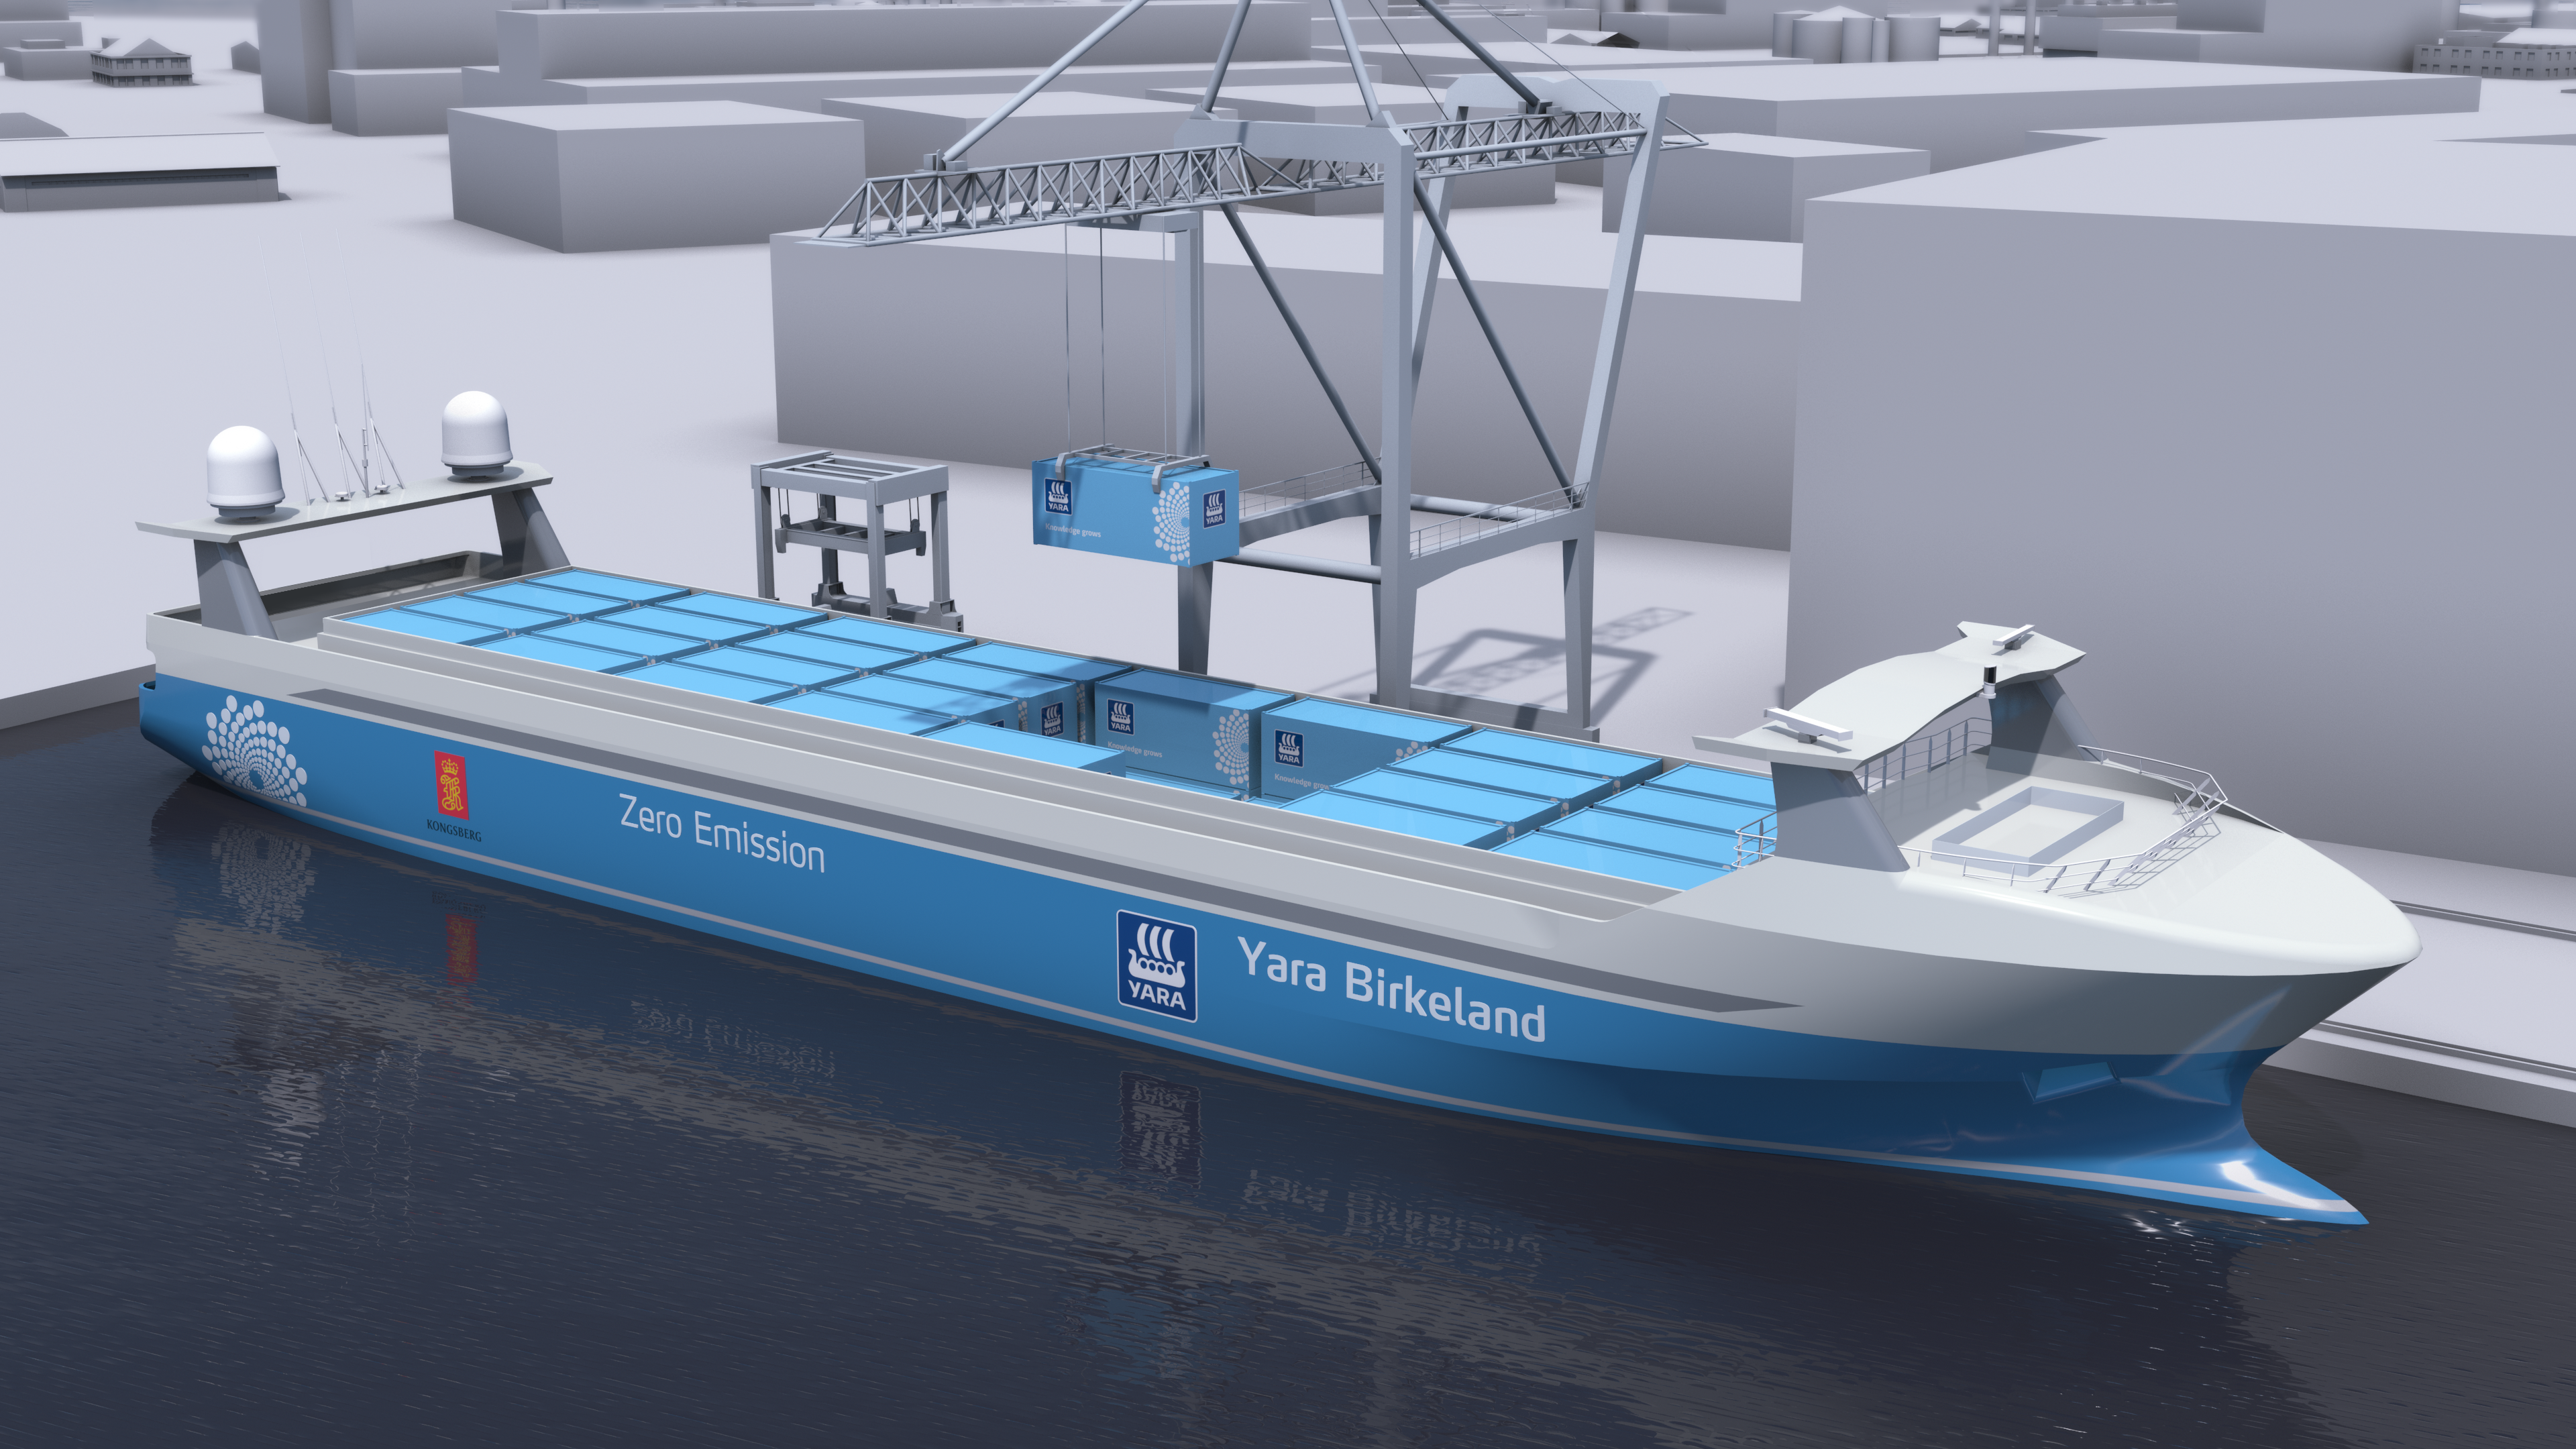
\includegraphics[width=\textwidth]{yara-birkeland.png}
	\caption{Render of Yara Birkeland}
	\label{fig:yara-birkeland}
\end{figure}

Other smaller projects are the development of Norwegian ferries, which are likely to start sailing automated from 2018, just like an automated shuttle service for offshore installations. A partly Dutch project is the Roboat, where a fleet of small pontoons will be used to solve problems on urban waterways. Such as transportation of people and goods, or creating temporary dynamic floating structures like bridges and stages. Roboat is a collaboration between AMS Institute and MIT.

Most of the previous projects focussed on developing a vessel, which has to operate in the current environment. The smart shipping challenge (SMASH) focusses on combining technological developments within different parts of the inland shipping industry in the Netherlands, such as bridges and terminals. This will help to steer ships remotely, enable the intelligent exchange of information, and the optimisation of waterway maintenance.
Good examples are the new vessels from Nedcargo and the Gouwenaar 3. These vessels will be able to transport more containers while reducing fuel consumption. This will not only be acquired by improving the hull shape and machinery, but also by sailing smarter. For example by optimising the speed, based on opening times for bridges and availability of the quay \cite{SMASH2017}. 

Also in the Netherlands are different partnerships working on the challenges of autonomous and unmanned shipping. The research conducted on communication and decision making will support one of these projects via Damen Shipyards and the Technical University of Delft. Where they partner with different European companies and research institutes, to develop a technology to deal with challenging environments and complex transport missions. Which is also applicable to other autonomous waterborne operations, such as inland waterways transport and coastal/inter-island short range ferry services.

Based on the projects mentioned above, are the most direct use cases: Local transport between factories and terminals and short sea shipping solutions. However, there might be more in the future, such as the usage of tugs as an additional actuator in dynamic positioning systems.

\section{Stakeholders}
When the ships mentioned in the previous section will sail, does not only dependent on the rate on which the technology can be developed. As stakeholders are there also regulatory bodies, such as \ac{IMO} and classification societies which need to incorporate autonomous vessels into their frameworks. 
The exploratory projects are important, as this will help them to prioritise the codes for different ship types. These codes include information on autonomy levels and how to certify unmanned vessels.

Another group of stakeholders are the shipbuilders, system integrators and suppliers for subsystems. These are responsible for technological development. More and more shipyards try to get involved, to gain knowledge on the development process. 
Also are there the companies from other industries, which see opportunities for products they already developed for planes or automotive. For example using computer vision, protocols for classifying systems and connecting ships.

The last, but probably most important are the customers, as technology will only be used if they can make money with it. More and more companies are convinced this is possible. These are not only the chartering companies but also their customers, such as Heineken, Yara and BHP.

\section{Challenges when combining unmanned and manned vessel}
\label{sec:challenges-future}
Based on the projects mentioned above it is clear that many projects work on different challenges. All challenges are related to the safe operation of unmanned vessels while optimising profit. For the technological challenge, is the most critical situations, when manned and unmanned vessels meet. Ship-to-ship communication is often necessary for those situations. Many of the projects so far, try to avoid these situations, as this will also result in fewer challenges for regulatory bodies. Also is technology for communication costly to develop, therefore is the aim to avoid communication where possible. The first step to accomplish this is to adjust the operational strategies for unmanned ships to avoid complex situations. This means that a strategy should be developed on how these ships can avoid communication. The easiest way is to operate only in area's where all risks are known. The best solution to enable a ship to operate everywhere is by avoiding the need for communication. This is achieved by taking decisions well in advance and making intentions clear. Still, some challenges are open, as ships cannot avoid all complex situations. For these cases, there must be a protocol which enables manned and unmanned ships to share the right information. Both of these issues have not been within the scope of the previously mentioned projects, or any other research \cite{Kooij2018}. 

\vspace{1.5cm}
\emph{In the next chapter} are factors discussed which influence the decision making process. We base these factors on challenges from previously mentioned projects and current research, where the decision model is a stepping stone.
\chapter{Decision model for safe operation}
\label{ch:model}
In the previous chapter, several projects are discussed, that gave insight in the challenges towards unmanned and autonomous shipping. To gain insight into the challenge of communication is a decision model used. This model shows which factors influence the decision-making process and how relevant research support this. The steps in this decision process are the same for manned and unmanned ships.
The decision process within the model is based on Boyd's OODA loop \cite{Boyd1987}, Endsley model for situational awareness \cite{Endsley2013}, and combined with models used in the projects as mentioned in chapter~\ref{ch:future}. 
The OODA loop has different phases: Observe, orient, decide and act. Similar to Endsley's model: Perceive, comprehend, project, decide and act. 

The combined model describes how this applies to choosing the right strategy for safe operation, and relates to external factors and relevant theory. Figure \ref{fig:decision-model} illustrates the decision model used in this research, this model shows the multiple phases in the decision process. The first step describes what can be observed, to form a mental model. The next step is to orient, which is divided into the identification of the situation and the identification of future hazards. This step will result in a set of strategies, which will be evaluated using different criteria, resulting in a decision. After this decision, the operator administers an action. This action finally results in a new situation, observed in the next iterative step. This chapter will discuss these phases in more detail and how they relate to the challenge of communication, by discussing external factors and relevant theory.

\begin{figure}[p]
	\centering
	\includegraphics[width=\textwidth]{decision-model.png}
	\caption{Decision model}
	\label{fig:decision-model}
\end{figure}

\section{Decision process}
The decision process is the core of this model. Part \ref{part:MT} will use the decision process on a less abstract level than described in this chapter. The steps taken in this decision process are similar for manned and unmanned vessels. Their way of thinking differs however when this is related to being consistent or handling exceptions.

\subsubsection{Mental model}
The first phase of the decision process is to form a mental model. A mental model is a representation of the surrounding world, including the relationships between its various parts and a person's intuitive perception about his or her acts and their consequences.
Sensor data about the environment is used to make this representation. Systems interpret raw data, transforming it into information, which can be combined into knowledge. 

The steps from sensor to knowledge still require much research, although large steps are taken within the domains of LIDAR \cite{Cameron2017}, computer vision \cite{Marr2017} and sensor fusion \cite{Hoffman2018}. Appendix \ref{app:systems} discusses the systems which are used at the manned vessel, to form a correct mental model. For this research, only the result of this step is relevant: Is the acquired knowledge sufficient to identify the situation correctly, or is more information needed?
Future technologies and sensors are not within the scope of this research, nor how their outputs result in useful information. 

\subsubsection{Identify situation}
The step from information to knowledge is in the phase where the situation, scenario, and hazards are identified. How this would go in practice is discussed in chapter \ref{ch:identify-situation}. This step identifies critical situations during the design phase of an autonomous ship to be evaluated. 
This research will define a method to evaluate these critical situations. The layout of the waterway, other nearby vessels, relevant regulations, etc. determines the situation and scenario.

\subsubsection{Predict future states and decide on strategy}
Based on the situation, different strategies might be possible. A system or the operator has to evaluate these strategies. This evaluation is done by predicting how different strategies will influence the path of the various vessels. A trade-off must be made between exact calculations and computation time. For example is the \acf{CPA} currently determined using linearised algorithms in common \ac{ARPA} systems. Non-linearised methods using, for example, a Bézier curve will result in smaller errors. Simulations would improve this even more, however, does a simulation with correct hydrodynamic models cost much more computational time. In chapter~\ref{ch:criteria-problem}, the linearised and non-linearised methods are described. Appendix \ref{app:tool} describes the simulation tool. This tool is however not optimised for such calculations. Therefore these calculations cannot be done real-time. The hydrodynamic model used in the simulation is also described in appendix \ref{apps:hydro-model}. Different manoeuvres are evaluated after this phase, that correspond to the different strategies. We will discuss this in chapter \ref{ch:criteria-manouvre} for common critical strategies. This will result in manoeuvring requirements. These requirements can be used by ship designers, to ensure that the ship can operate safely with minimal need for communication.
After the evaluation of these criteria is known which strategy will result in safe operation of the vessel.

\newpage
\section{External factors}
How easy it is to go through the decision process and end up at the right strategy depends on the situation. Environmental factors, such as the traffic situation, will mostly influence the situation. In some cases are the static sensors not sufficient to analyse the environment properly, resulting in an incomplete mental model. This section will describe in more detail how the environment influences the forming of the mental model and how safe operation within this environment would benefit from communication. 

\subsection{Environment}
The mental model is a representation of the environment in which the vessel acts. The sensors will measure this environment and provide the data. Many critical situations occurred due to weather conditions. The cause is that sight is limited during heavy rain or snow. The wind and waves might limit the manoeuvring capabilities of a vessel. These are also the reason that some vessels are not allowed to enter a port when wind or waves are too high.
If such repercussions are necessary, depend on the layout of the waterway. Due to currents, operations (e.g. maintenance and fishery) or limited depth, might some area's be restricted. Operators acquire this information via communication channels, but communication channels which only allow receiving and not sending, such as \acf{Navtex}.

The same applies to standard information on other ships. They might send their location and speed via \ac{AIS}, but still key is the \ac{ARPA}. Due to weather conditions, these systems can be less accurate, as heavy rain results in noise at the radar. In the situations where sensors do not function as expected, communication is needed, even if the whole decision process itself is optimised to avoid communication.
The same goes for communication with shore-based stations such as traffic controllers or in the future remote pilots. Sensors or current systems are not able to retrieve this information. Such as a place and time to berth or pick-up a pilot.

Both shore-based stations and ships can only share intentions and their planned path via the radio. Future unmanned will most likely be able to negotiate using other systems. But in the case with manned-manned or manned-unmanned interaction is this only possible via \ac{VHF} radio for now.

\newpage

\subsection{Communication}
As described there are still cases in which communication is necessary. We discuss in part \ref{part:CS} a case where communication between manned and unmanned vessel is needed. Using the \acf{sCE} method a protocol is defined, based on existing systems and protocols. Thus using \ac{AIS} to send written messages, or \ac{VHF} and \ac{SMCP} for verbal messages. 
Other cases such as communication with traffic controllers and pilots could use the same protocol. Although they might need to share more information with unmanned vessels, which could be done with a new system such as \ac{VDES}. This will however not be part of this research.


\part{Effect of manoeuvrability on decision making}
\label{part:MT}
\chapter*{Introduction}
\label{sec:introduction}
\addcontentsline{toc}{chapter}{Introduction}

The Maritime industry is tapping into the world of automation and digitalisation. The automation level of vessels is proliferating. Vessels are getting connected to the shore by different means. Operational data is becoming available and enriched with other data sets like design data, weather data and maintenance data. These technologies boost the development of autonomous and unmanned vessel designs \cite{Blanke2017}. 
At the same time is the Maritime Industry facing challenges when it comes to crewing and safety \cite{Cappelle2018}. Combined with an increasing competition it is hard to make healthy margins. These trends trigger Maritime Industry to embrace autonomous sailing technologies to secure a healthy future. These business developments reflect in the significant amount of research and development projects \cite{SMASH2017} \cite{Eriksen2017} \cite{MUNIN2016} \cite{Sames2017} \cite{RollsRoyce2015} \cite{Waterborne2016}. Each one of these projects tackles one or more challenges in the development of autonomous sailing. However, is the challenge of communication between unmanned and manned vessels not been tackled \cite{Saarni2018}. In chapter~\ref{ch:future}, these challenges and related projects are discussed. Currently, no solutions are available. However, this is necessary to ensure the safety of all vessels: manned, unmanned, remote, automated and autonomous.

This report presents the results of the research on communication between unmanned autonomous sailing vessels and manned vessels. It gives a design philosophy which has been translated in a methodology for handling communication which is eventually turned into protocols which are derived based on theory and validated through simulations.

% More people start to believe in the possibilities of unmanned and autonomous shipping, as there are many projects which try to develop the necessary technologies \cite{SMASH2017} \cite{Eriksen2017} \cite{MUNIN2016} \cite{Sames2017} \cite{RollsRoyce2015} \cite{Waterborne2016}. The major reason for the development of autonomous ships are the benefits for operational expenses. But one of the major reasons for acceptance is the mitigation of human errors. Which can be achieved by taking out humans from the chain of command. This will, however, introduce new challenges \cite{Saarni2018}. In chapter \ref{ch:future} these challenges and corresponding projects are discussed. One of the less explored challenges is the issue of communication. This becomes harder between manned and unmanned vessels. Communication is used to share information on the intentions or discuss future actions. At the moment there is no protocol which can be used by unmanned vessels. However this is necessary to ensure the safety of all vessels: manned, unmanned, remote, automated and autonomous.
% To solve this challenge, there are two possibilities: Avoid the need for communication, or develop a new communication protocol.

\subsubsection*{Context}
In many situations is the \acf{COLREGs} sufficient to determine the intentions of other vessels \cite{IMO1972}. They can be seen as ship separation rules, which guide all vessels to make early and correct alterations to their course. It will take more time to assess the situation when using \ac{VHF}. Meaning there is less time to act, which limits the possible strategies. These rules do also apply to autonomous ships, and thus can be used when manned and unmanned vessels meet.
Examples are to stay on the starboard side of the shipping lane, and not to cross other ships with a small relative angle. When this does not happen, communication is necessary. When this communication doesn't occur correctly, there is a much higher risk of accidents (appendix \ref{app:accidents}). Thereby are there also situations in which regulations are contradictory, such as the accident between Artadi and St-Germain as described in appendix \ref{sec:artadiVSst-germain}. These contradictions occur more often in complex situations, such as a harbour approach.

The risks when \ac{COLREGs} are not sufficient can be mitigated by taking decisions, well in advance. What well in advance means, depends on the manoeuvrability and operation of a vessel. A cargo vessel will follow common paths, while a small tugboat might move around much more. These situations result in more false positives on potential collisions with other vessels, when using the same safety domain and evaluation system. The impact of manoeuvrability means that it is necessary to think ahead several minutes with a large ship, while this is much shorter for a small tugboat. This time-domain for decision making depends not only on the ship characteristics but also on the waterway characteristics. Chapter~\ref{ch:model} discusses this in more detail. Examples are the depth, traffic separation schemes and harbour entrances.

If it is not possible to take decision well in advance, it is often due to a lack of information. Communication solves this problem. This communication between manned vessels happens in different ways. Most important is communication via \ac{VHF}, thereby is information from the AIS used to identify ships. Also can this information help to determine the intentions of the vessel, based on the type of vessel or destination. The used protocols for these systems are discussed in appendix~\ref{app:systems}

\subsubsection*{Design philosophy}
We developed a strategy to cope with the challenge of communication between manned and unmanned vessels, without introducing new systems to the bridge of manned vessels. 
First, we will try to avoid the need for communication, by staying well clear from other ships. When this is not possible, there is a need for communication. A new protocol must be developed for this communication.
This strategy can be used as a foundation to build a system for decision making which ensures safe operation of both manned and unmanned vessels. Different steps must be taken to implement this strategy. 

First insights have been acquired on the decision model for safe navigation, to determine which factors are taken into account to make a decision. The next step is to learn how these factors influence the decision process. This can also be used to determine the critical situations. Showing when it isn't possible to navigate without communicating. Leaving some specific situations for which a communication protocol must is necessary. Using the \acf{sCE} method, the operational demands, relevant human factors and envisioned protocol could be defined. The current state of the maritime industry is taken into account.

\subsubsection*{Research questions}
The report will touch upon different research domains in more detail: Maritime Technology and Computer Science. The part on maritime technology focuses on the situation where manoeuvring is just enough. While the computer science part will focus on the development of the communication protocol. Answering the following research questions:

\begin{quotation}
	\emph{How do ship manoeuvrability characteristics influence the domain for decision making, to ensure that the chosen strategy will result in a passing distance which does not require communication?} 
\end{quotation}

\begin{quotation}
	\emph{Will a protocol based on existing maritime systems and communication protocols be sufficient to ensure safe navigation, while manned and unmanned vessels encounter each other?}
\end{quotation}

\subsubsection*{Report structure}
This research has three parts. In those parts, the challenge of communication between manned and unmanned vessels is considered. Part~\ref{part:general} gives a more detailed context of autonomous shipping. This context is used with a decision-model to show why communication is a challenge, and how this challenge can be tackled.

Part~\ref{part:MT} aims to determine how communication can be avoided. To resolve this, it is important first to determine when communication is necessary, which is in case of critical situations. These situations are tested in a simulation environment. The time-domain for decision making can be determined to ensure safe operation in these simulations. These situations are simulated, using a validated manoeuvring model. Thereby is evaluated that ships need communication in fewer cases if the decision-domain is improved.

Part \ref{part:CS} will focus on critical situations where communication is a must. Currently, a communication protocol between manned and unmanned vessels has not been part of any known project. Communication is necessary in cases where there is a lack of trust, missing information or the time-domain for decision making becomes critical. To ensure a fest implementation of the communication protocol between manned and unmanned vessels, will it be based on existing systems and protocols. The aim of this part is to validate if it is possible to define a protocol using the \acf{sCE} method, which will be accepted by seafarers.

\chapter{Decision making process}
\label{ch:decision-process}
Using a rule-based time-domain decision model, can a general decision process be defined to make insightful: What the situation is and what problem might occur. Nodes in the decision tree are described with keywords to work in a structured way. This white-box approach will cover as much as possible, however is it likely to use machine learning in the final design of a decision algorithm for autonomous and unmanned ships. First the decision phases are described. Followed by lists of nodes used to identify scenarios and situations. Combining this with the rules, will result in the decision model. Also the criteria necessary to go trough the steps are discussed. The aim of this decision model is gain insight in the decision process to show what critical situations are when you want to try to avoid communication.

\section{Decision phases}
The decision making process has different phases. This can be seen in the process diagram how these phases relate. This is shown in figure \todo{add process diagram}. These different phases are also described in table \ref{tab:phases-description}.
\begin{table}[H]
	\begin{tabular}{p{0.35\textwidth}|p{0.64\textwidth}}
		\toprule
		Class & Description\\
		\midrule
		Mental model & Acquire knowledge about the situation, not part of this research \\
		Situation identification & Identify the encountered situation, to determine which criteria are relevant, based on waterway lay-out and other ships. \\
		Predict future states & The second step is to determine if a problem will occur, as there is only a change in strategy needed when this is the case. \\
		Strategy & If there is a problem, a new strategy should be chosen, this is based on the evaluation of criteria. \\
		Action & From this strategy, different actions will follow. \\
		Result & Finally the result is evaluated, using the same criteria to determine a problem in future states. \\
		\bottomrule
	\end{tabular}
	
	\captionof{table}{Description of phases in decision process}
	\label{tab:phases-description}
\end{table}

\section{Nodes in decision making tree}
To describe the nodes within the decision trees, short keywords are used. These describe in short what kind of situation, problem, strategy, action or result there is. By using the same terms, confusion is avoided. Definitions for those terms are given in this section.

\subsubsection{Encountered situations}
This is the first step to limit the amount of strategies which are relevant to evaluate. The nodes within the identification process are described in table \ref{tab:situations}, more details on how this is determined is described in section \ref{sec:situation-identification}.
\begin{table}[H]
	\begin{tabular}{p{0.35\textwidth}|p{0.64\textwidth}}
		\toprule
		Tag & Description\\
		\midrule
		Passing & The paths of both ships are in opposite direction, and do not cross. \\
		Crossing & The final direction of both ships differs, but they do cross. \\
		Merge & The final direction of both ships is the same. \\
		Over-taking & The paths of both ships are the same but at different speeds. \\
		\bottomrule
	\end{tabular}
	
	\captionof{table}{Tags for different situations}
	\label{tab:situations}
\end{table}

\subsubsection{Predict future states}
To identify if a problem will occur, different criteria are being evaluated. These criteria are described in chapter \ref{ch:criteria-problem}. In table \ref{tab:identification-criteria} the nodes within the decision tree are discussed to evaluate if there is a problem, and what kind of problem there is. 
\begin{table}[H]
	\begin{tabular}{p{0.35\textwidth}|p{0.64\textwidth}}
		\toprule
		Tag & Evaluation \\
		\midrule
		Closest point of approach & Good; Too close \\
		Crossing point & In front; Behind \\
		Crossing distance & Good; Too close \\
		Relative speed & Faster; Same speed; slower \\
		\bottomrule
	\end{tabular}
	
	\captionof{table}{Criteria and result of evaluation to determine problem}
	\label{tab:identification-criteria}
\end{table}

\subsubsection{Possible strategies}
Using the identification of the situation and prediction of future states. A limited number of strategies might be possible. The strategies will result in actions, but can be categorized in the groups as described in table \ref{tab:strategies}.
\begin{table}[H]
	\begin{tabular}{p{0.35\textwidth}|p{0.64\textwidth}}
		\toprule
		Tag & Description\\
		\midrule
		Follow planned path & By doing planned actions \\
		Move away from other path & Change path, in order to increase CPA\\
		Stay parallel for longer & Change path, to sail parallel to other vessel \\
		Adjust speed & Slow-down or speed-up\\
		Abort over-taking & Lower speed and stay behind other vessel \\
		Move away from other position & Check if this is to starboard, otherwise communicate \\
		Communicate & If other (also) has to take action to avoid a problem \\
		\bottomrule
	\end{tabular}
	
	\captionof{table}{Tags for different strategies}
	\label{tab:strategies}
\end{table}

\subsubsection{Possible actions}
From the chosen strategy, different actions will follow. These action are a combination of an action type, and a moment to execute action. In table \ref{tab:actions} and \ref{tab:time-domain-action} these are described. The criteria to determine if an action is possible are described in \ref{tab:manouvre-criteria}.
\begin{table}[H]
	\begin{tabular}{p{0.35\textwidth}|p{0.64\textwidth}}
		\toprule
		Tag & Description\\
		\midrule
		Continue without change & Do not change speed or rudder\\
		Evasive manoeuvrer to starboard & Steer starboard first and end at same course\\
		Evasive manoeuvrer to portside & Steer to portside first and end at same course\\
		Slow down & Reduce speed\\
		Speed-up & Speed-up \\
		Emergency stop & Turn ship side-ways and set propulsion in reverse\\
		Communicate & Discuss required actions with other vessel(s)\\
		\bottomrule
	\end{tabular}
	
	\captionof{table}{Types of actions}
	\label{tab:actions}
\end{table}

\begin{table}[H]
	\begin{tabular}{p{0.35\textwidth}|p{0.64\textwidth}}
		\toprule
		Tag & Description\\
		\midrule
		Now & When action can be undertaken as soon as possible \\
		In ... minutes/seconds & Wait for a period of time to ensure bold movement \\
		After action ... & Wait with action till you or other has done another action \\
		\bottomrule
	\end{tabular}
	
	\captionof{table}{Time-domain for action}
	\label{tab:time-domain-action}
\end{table}

\begin{table}[H]
	\begin{tabular}{p{0.35\textwidth}|p{0.64\textwidth}}
		\toprule
		Tag & Evaluation \\
		\midrule
		Closest point of approach & Good; Too close\\
		Time till problem & ... minutes/seconds\\
		Distance till problem & ... meter \\
		\bottomrule
	\end{tabular}
	
	\captionof{table}{Criteria to determine if action is possible}
	\label{tab:manouvre-criteria}
\end{table}

\subsubsection{Result}
Using the evaluations from the action phase, can the eventual solution be evaluated. Herein is the human factor on board of other vessels taken into account, in the form of perceived risk. Evaluations and criteria are shown in table \ref{tab:criteria-safe-situation}.
\begin{table}[H]
	\begin{tabular}{p{0.35\textwidth}|p{0.64\textwidth}}
		\toprule
		Tag & Evaluation\\
		\midrule
		CPA & Good; Too close\\
		Perceived risk & Safe; Uncomfortable; Close encounter; Too close\\
		Safe situation & Yes; Uncomfortable; No\\
		Communicate & Yes; No\\
		\bottomrule
	\end{tabular}
	
	\captionof{table}{Tags for safe situation criteria}
	\label{tab:criteria-safe-situation}
\end{table}


\section{Critical paths in decision trees}
When combing the nodes as described in the previous section, very large decision trees are obtained. For specific situations and scenarios the eventual decision tree is much smaller than a tree covering all possibilities. 
Therefore the decision trees are split up per phase. Examples of these trees can be found in appendix \ref{app:decision-trees}. Several common critical paths within those trees can be identified. These paths will be used in later chapters to evaluate criteria, manoeuvring requirements and eventually do a case study.







\chapter{Identification of situation and scenarios}
\label{ch:identify-situation}
The start of the decision tree as described in chapter~\ref{ch:decision-process} is the identification of the situation and scenario. This identification aims to narrow down possible strategies in the next phases of the decision making process. In this chapter, the first steps of classifying the situation are discussed. Followed by the steps taken in the orientation phase to form strategies. Which will help to determine which paths are common and critical, thus are good to be used while evaluating manoeuvring criteria.

\section{Situation identification}
\label{sec:situation-identification}
Situations can be classified into four types. These are also discussed in chapter~\ref{ch:decision-process}, as these are the same as the nodes in the decision tree:
\begin{description}
	\item [Passing] The paths of both ships are in opposite direction, and do not cross.
	\item [Crossing]The final direction of both ships differs, but they do cross.
	\item [Over-taking] The paths of both ships are the same but at different speeds.
	\item [Merge] The starting direction of both ships differs, but the final direction is the same.
\end{description}
It depends on the waterway lay-out which situation is likely. This can be influenced by traffic separation schemes, forbidden zones or land masses. To determine the situation, a classification of paths is used. To do this systematically, paths will be based on figure~\ref{fig:junction-letters} and can be written as: [current~position,~direction].

To classify a situation where two vessels encounter each other, the paths are considered. Key is to determine the angle between those paths. This way it is possible to classify them using table~\ref{tab:scenarios-standard}.

\begin{minipage}{\textwidth}
	\begin{minipage}[b]{0.62\textwidth}
		\centering
		\begin{tabular}{l|l|l}
			Own ship & Other ships & Situation\\
			\hline
			\big[A,D\big] & [D,C] [D,B] [D,A] [C,B] & Passing \\
						  & [C,A] [B,A] [B,C] & \\
			\big[A,C\big] & [C,A] [C,B] [B,A] & Passing \\
			\big[A,B\big] & [D,C] [C,D] [B,A] & Passing \\
			\big[A,C\big] & [D,B] [D,A] [C,D] [B,D] & Crossing \\
			\big[A,B\big] & [D,A] [C,A] [B,D] [B,D] & Crossing \\
			\big[A,D\big] & [C,D] [B,D] & Merge \\
			\big[A,C\big] & [D,C] [B,C] & Merge \\
			\big[A,B\big] & [D,B] [C,B] & Merge \\
			\big[A,D\big] & [A,D] & Over-taking \\
			\big[A,C\big] & [A,C] & Over-taking \\
			\big[A,B\big] & [A,B] & Over-taking \\
		\end{tabular}
		\captionof{table}{Path definitions for different situations}
		\label{tab:scenarios-standard}
	\end{minipage}
	\hfill
	\begin{minipage}[b]{0.37\textwidth}
		\centering
		\includegraphics[width=\textwidth]{junction-letters.png}
		\captionof{figure}{Path description \\ for situation identification}
		\label{fig:junction-letters}
	\end{minipage}
\end{minipage}

The boundaries to determine if the other ship comes from direction A, B, C or D are based on \ac{COLREGs} \cite{IMO1972}. Direction A is between 112.5 and 247.5 degrees, as shown with the dotted line in figure~\ref{fig:junction-letters}. While sailing this angle can be observed using the mast-head lights. Which are seen as red when the vessel comes from B, green when from D and green and red from C. While from direction the color of the light will be white. The other situation which might be difficult is when a ship comes from the front with an angle. When in doubt if it is a head-on situation or a crossing situation. Always assume a head-on situation, as this stated in rule 14 \cite{IMO1972}.

\section{Situations which limit possible strategies}
Beside this first identification of the situation. More details must be taken into account to eventually form the right strategies, as these details might limit the possible strategies. Below the effect of the waterway and actors are discussed on possible strategies.

\subsection{Waterway properties}
To limit the strategies which have to be evaluated, are strategies filtered based on the physical properties of the waterway. As this might restrict the area where can be sailed, which influences the possible strategies. For example is it common to over-take ships in open-water on starboard side. While on restricted waterways ships will sail as far as possible to starboard already. This means the ship which is over-taking will have to pass on the port side of the other vessel, at the center of the waterway.

In the next step other static hazards are considered to check if the chosen strategy does not lead to a collision. Or if there are specific regulation frameworks for this waterway. These are however not part of the first iteration of the decision model, as this will introduce much more complexity, without improving the result in most cases. Examples of static hazards which could be evaluated in future iterations are bridges, buoys, forbidden zones, quays, port mouth or shallow waters. As possibilities for over-taking or evasive manoeuvers are limited in those cases for example. This means the strategies are limited.

Another limiting factor related to waterways are the difference in regulations between waterways. Most obvious are traffic separation schemes, or other road marks such as signs which forbid to over-take or meet. But others are for example to not create wash or no turning, thus limiting the options to manoeuvrer. Or more directive signs on obligated directions or speed limits. This is mostly relevant for coastal and inland waterways.

\subsection{Dynamic objects}
The second major step is the identification of dynamic objects. Those are all relevant moving objects. Most obvious are off course other ships which do come close. But in future developments of the decision model, objects which are not under any control of a human should also be considered, such as floating containers. The major difference between static hazards are of course that the 'forbidden zone' around these objects change over time. This means more complex evaluation methods are needed to determine if there is no perceived risk, and thus a safe situation.

These complex evaluation methods will have to predict the path. To dot this, first the general information about the object should be acquired. Such as manoeuvrability, speed, course, type of object, under control, etc.
Thereby might it be possible in future developments to take into account the human factor to improve the path prediction. This could be based on the experience of the crew, availability of a pilot or if the vessel is completely unmanned.

Examples of such dynamic objects which limit the possible strategies are for example fishery vessels. As they might have long nets behind them while in operation. Ferries in inland waters which have priority over other shipping traffic. Other ships with limited manoeuvrability or forbidden zones around them. As these all could force to act on a specific strategy.

\section{Scenarios}
Using the information about the properties of the waterway and actors, the scenario can be identified. Where the situation is based on observations and describes the current state. Do the scenarios take into account the possible future strategies of those actors and thus describe what the future states could be.
Based on the scenarios, can be determined which rules to apply and what their implications are on the possible strategies. The same goes for the estimated path of dynamic objects. This might also narrow down the possible strategies.

Using the above mentioned information in the decision model, the strategies can be narrowed down. This can be used to simplify the decision tree and select the right criteria to evaluate.
Different scenarios for the same situation could be that the ship turns to port or starboard. For both does a probability exist. Using a probability index for the decision of other vessels will in this case improve the eventual decision making. This can be taken into account by for example the safe motion parameters as described by Szlapczynski \cite{Szlapczynski2017}.

\vspace{1.5cm}
\emph{In the next chapter} the criteria are defined to evaluate the situations and scenarios. This evaluation shows if a problem might occur. These criteria are eventually used to determine the most critical common situations. 


\chapter{Definition of criteria for evaluation of situation}
\label{ch:criteria-problem}
To determine whether a problem might occur in the situations and scenarios as identified in the previous chapter, different criteria are evaluated. The current systems calculate most of these criteria, such as \ac{ECDIS} and \ac{ARPA}. However, they do use linearised algorithms. These do not predict the \ac{CPA} and crossing distance correctly while turning, often resulting in many dismissed alarms. This chapter describes different criteria, followed by the calculation needed to evaluate these criteria. This description and calculation are given for both the linearised algorithms and proposed algorithms. Later in the process, these criteria can be used again, to ensure that the chosen strategies ensure safe operation with low perceived risk.

\section{Calculations based on current systems}
\label{sec:linearised-methods}
Within \ac{ARPA} and \ac{ECDIS}, different calculations are made, which can be used to evaluate if there is a problem in the current scenario. These calculations often use linearised algorithms, which results are not correct when turning. Humans can easily dismiss the false alarms given due to these wrong results. Computers do not handle these false positives well. The advantage, however, is that the calculations can be done very fast. Below these calculations are discussed for the \acf{CPA} and crossing position.

\subsection{Closest point of approach}
The \ac{CPA} refers to the positions at which two dynamically moving objects reach their closest possible distance, which is an important calculation for collision avoidance. A linearised form uses two points moving at fixed speed and fixed direction. Figure \ref{fig:CPA} shows an example, where P and Q are the moving points, with corresponding direction vectors $u$ and $v$, which include the speed and direction.

\begin{figure}[h]
	\centering
	\includegraphics[scale=0.6]{CPA_lines.png}
	\caption{Example for \acf{CPA}}
	\label{fig:CPA}
\end{figure}

A formula can be derived for the closest point of approach. With the motion equations for $P$ and $Q$, the distance can be calculated. Where $P_0$ and $Q_0$ are the current positions, and $u$ and $v$ are the corresponding speed vectors:
\begin{equation}
\label{eq:motion}
P(t) = P_0 + t \cdot u ;\quad  Q(t) = Q_0 + t \cdot v
\end{equation}
\begin{equation}
d(t) = |P(t) - Q(t)| = |P_0 - Q_0 + t (u - v)|
\end{equation}

Since d(t) is a minimum when $D(t) = d(t)^2$ is a minimum, this is the case when the derivative is equal to 0:
\begin{equation}
D(t) = d(t)^2 = (u - v) \bullet (u - v) t^2 + 2 (P_0 - Q_0) \bullet (u - v) t + (P_0 - Q_0) \bullet (P_0 - Q_0)
\end{equation}
\begin{equation}
\frac{d D(t)}{dt} = 0 = 2t[(u - v) \bullet (u-v)] + 2 (P_0 - Q_0) \bullet (u - v)
\end{equation}

This equation can be solved for t, to calculate the moment where CPA is the smallest:
\begin{equation}
\label{eq:t_CPA}
t_{CPA} = \frac{-(P_0 - Q_0) \bullet (u - v)}{|u - v|^2}
\end{equation}
\begin{equation}
d_{CPA}(t_{CPA}) = |P_0 - Q_0 + \frac{-(P_0 - Q_0) \bullet (u - v)}{|u - v|^2} \bullet (u - v)|
\end{equation}
If $t_{CPA}$ is smaller than 0, the CPA is in the past. If $t_{CPA}$ is equal to 0, the CPA is right now, else it is in the future. If $u$ and $v$ are the same, the denominator of equation~\ref{eq:t_CPA} is equal to 0. This means that the CPA is constant.

\subsection{Crossing distance}
The crossing distance is the distance between two ships if they pass each others path. The position of another vessel can be both in front or behind a vessel. This distance is mostly relevant for how safe a crossing situation feels. The crew on manned ships do not want to have ships too close in front of them, as they can't do an evasive manoeuvrer in those situations. The same motion equation as for CPA can be used (equation \ref{eq:motion}). 

\begin{figure}[h]
	\centering
	\includegraphics[scale=0.6]{crossing_lines.png}
	\caption{Example for crossing point and distance}
	\label{fig:crossing-distance}
\end{figure}

In figure \ref{fig:crossing-distance} the distance is calculated between two points at a certain moment in time. The first step is to calculate the crossing point (cp) of the two lines:
\begin{equation}
P(t_{cp,p}) = Q(t_{cp,q}) \rightarrow P_0 + t_{cp,p} \cdot u = Q_0 + t_{cp,q} \cdot v
\end{equation}
\begin{equation}
t_{cp,P} = \frac{(Q_0 - P_0) \times v}{u \times v}
\end{equation}
\begin{equation}
t_{cp,Q} = \frac{(P_0 - Q_0) \times u}{v \times u}
\end{equation}
\begin{equation}
cp = P_0 + \left[ \frac{(Q_0 - P_0) \times v}{u \times v} \right] \cdot u =  Q_0 + \left[ \frac{(P_0 - Q_0) \times u}{v \times u} \right] \cdot v
\end{equation}

The next step is to determine where each vessel is when the other vessel is at the crossing point. To determine finally what the crossing distance is:
\begin{equation}
P(t_{cp,Q}) = P_0 + \left[ \frac{(Q_0 - P_0) \times v}{u \times v} \right] \cdot u
\end{equation}
\begin{equation}
Q(t_{cp,P}) = Q_0 + \left[ \frac{(P_0 - Q_0) \times u}{v \times u} \right] \cdot v
\end{equation}
\begin{equation}
d(t) = |P(t) - Q(t)|
\end{equation}
The crossing distance (cd) for when P crosses Q and vice versa, can be calculated using the following formulas:
\begin{equation}
d_{cd,PQ}(t_{cp,P}) = |P(t_{cp,P}) - Q(t_{cp,P})|
\end{equation}
\begin{equation}
d_{cd,QP}(t_{cp,Q}) = |P(t_{cp,Q}) - Q(t_{cp,Q})|
\end{equation}

\section{Proposed algorithm based on planned path}
Better non-linearised methods are necessary for the calculation of the \ac{CPA} and crossing point, to improve the evaluation of criteria. By predicting the likely path of a vessel, improved estimations can be made. These use a first-order change, based on the rate of turn and course. This prediction can be extended with a combination of expected location and the probability that another ship is choosing a specific strategy.

Although it will result in better evaluations, the disadvantage is that much heavier computations are required, while also introducing uncertainty with the numerical solver. 
The first step will be to make a combination of both the linearised and non-linearised methods. The calculations have to be done for every combination of ships.

The Bézier curve is used to describe the paths in a non-linearised manner. This section first defines a Bézier curve. Followed by the same criteria as in the previous section: \acf{CPA} and crossing distance. This time describing the algorithm using to calculate it in a non-linearised manner.

\subsection{Bézier curve}
The first iteration of the algorithm is semi-linearised, where the path of own ship is represented by a Bézier curve, based on its waypoints and strategy. Points have to be fitted along the planned path to describe the Bézier curve. This method is similar to the method as described by Taams \cite{Taams2018}. The path prediction for the other ship is still linearised, new systems and protocols have to be introduced to gather enough information on the strategy and waypoints.

For the calculation does the distance function not change. This is still $
d(t) = |P(t) - Q(t)|$. However is P taken as own ship and gets a new formula using the Bézier curve. This curve has a degree of $n$, which depends on the way-points and can be described using the following equations:
\begin{equation}
P(t) = \sum\limits_{i=0}^n b_{i,n}(t) \cdot P_i \quad and
\end{equation}
\begin{equation}
b_{i,n}(t) = \left( \begin{array}{c} n \\ i \end{array}\right) t^i(1-t)^{n-i}, i = 0,\dots,n
\end{equation}

\subsection{Closest point of approach}
\label{ssec:CPA-calculation}
The numerical algorithm used to calculate the CPA is shown below. Herein is the path of own vessel represented by a Bézier curve. While other vessels are represented with a linearised function as described in section~\ref{sec:linearised-methods}. This results in the following algorithm:
\begin{enumerate}
	\item Check if situation (course, speed, other vessels) has changed since last calculation:
	\begin{enumerate}
		\item No, break
		\item Yes, continue
	\end{enumerate}
	\item Use waypoints to determine expected path for own ship (Bézier curve).
	\item Use path to determine the location for each time-step.
	\item Use course and speed other ships to determine their location for each time-step
	\item Calculate distance between ships for each time-step:
	\begin{enumerate}
		\item If smaller than stored CPA, update stored CPA with calculated CPA
		\item If larger than stored CPA, do not update stored CPA
	\end{enumerate}
	\item Return CPA
\end{enumerate}

\subsection{Crossing distance}
The algorithm to calculate the crossing distance will require much less computational power, as not all time-steps have to be calculated. Just the ones where the paths cross. The following algorithm can be used. It should be noted that some calculations from the CPA calculation can be reused.
\begin{enumerate}
	\item Check if something has changed since last calculation:
	\begin{enumerate}
		\item No, break
		\item Yes, continue
	\end{enumerate}
	\item Use waypoints to determine expected path for own ship (Bézier curve).
	\item Determine crossing point(s) between linear path and Bézier curve.
	\item Check if crossing points exist:
	\begin{enumerate}
		\item No, break
		\item Yes, determine location for crossing point(s)
	\end{enumerate}
	\item Calculate time when ships are at crossing point(s).
	\item Calculate distance between ships at time of crossing.
	\item Return crossing distances.
\end{enumerate}

\vspace{1.5cm}
\emph{The next chapter} describes the criteria that depend on the manoeuvrability characteristics of a ship. Using the \ac{CPA} and crossing distance can be determined whether the chosen strategy without communication will result in safe operation. Where the algorithms as discussed in this chapter, will give more exact results.


\chapter{Manoeuvrability requirements for safe operation}

\section{Critical scenarios}

\section{Criteria}
Turning circle
Advance distance
Tactical diameter

\section{Resulting design matrix}

%\chapter{Analysis of scenarios}
\label{ch:scenario-examples}
Example scenarios will be discussed in this chapter. This is done to determine the relevance of criteria in different situations and scenarios. The same steps as described in the previous chapters will be taken to determine the right strategy. Situation sketches are used to support the descriptions. The results will be a list of tags for the specific scenarios, which can be used to identify a situation. These tags can than be linked to the different criteria.

\section{Entering Maasgeul towards North Sea, Rotterdam}
The first scenario which will be analysed, is from the viewpoint of a crude oil tanker, which will leave the port of Rotterdam. To enter the traffic lane towards the Maasgeul, it has to cross the path of another vessel coming from port-side. While taking another ship from starboard into account, which is already heading towards the Maasgeul.

The decisions which have to be taken are to change course and/or speed. This must be done multiple times. Different snapshots are taken throughout, including information on criteria which the crew uses to make their decisions.
This example case is made up, but is based on real situations as described by pilots and \ac{AIS}-recordings.
First a description of the situation is given, which is the starting point of this example. The aim of this description is to enable the reader to understand the situation.
Next relevant rules are discussed which should be taken into account when deciding on the strategy.
Followed by the different snapshots, which will give insight in the decision making process and relevant criteria. This is concluded with a calculations for the relevant criteria.

\subsection{Situation description}
The location of the situation is the junction between the Beerkanaal, Maasgeul, Nieuwe Waterweg and Callandkanaal. A map with more details is shown in figure \ref{fig:Maasgeul-situation-1200}. Quays restrict the possible paths ships can sail to avoid each other, there is however no traffic separation scheme. 
In this example case there will be three vessels involved. 
\begin{description}
	\item [GULF VALOUR] 249 meter crude oil tanker. Coming from the Yangtzekanaal, heading to the Maasgeul, via the Beerkanaal. Just rounding the pier of 8e Petroleumhaven with 7.8 knots.
	\item [ASTRORUNNER] 142 meter container ship. Coming from the Maasgeul with 13.4 knots heading towards the Calandkanaal.
	\item [ANGLIA SEAWAYS] 142 meter ro-ro cargo carrier. Leaving Rotterdam via Nieuwe Waterweg towards the North-Sea with 10.3 knots.
\end{description}

All ships have licensed pilots on board, thereby do traffic controllers monitor the traffic and might give directions.

In order to classify a situation, tags are used. Example tags for this situation are: 
\emph{junction, harbour, restricted waterways, multiple vessels, traffic controller}

\begin{figure}[H]
	\centering
	\includegraphics[width=\textwidth]{Maasgeul-situation-1200-start.png}
	\caption{Situation sketch 12:00, with area which can be observed by Gulf Valour}
	\label{fig:Maasgeul-situation-1200}
\end{figure}


\subsection{Relevant COLREGs}
The rules relevant for the situation are discussed, these should be taken into account during the decision making process, ordered in a chronological manner, on the moment it becomes relevant. 

\emph{Rule 7a: Every vessel shall use all available means appropriate to the prevailing circumstances and conditions to determine if risk of collision exists. If there is any doubt such risk shall be deemed to exist.} \\
This is particularly relevant in this case, as both ships can't be observed by the Gulf Valour by sight or radar at the start, due to port terminals and landmasses. 

\emph{Rule 19d: A vessel which detects by radar alone the presence of another vessel shall determine if a close-quarters situation is developing and/or risk of collision exists. If so, she shall take avoiding action in ample time, provided that when such action consists of an alteration of course, so far as possible the following shall be avoided:\\
	(i). an alteration of course to port for a vessel forward of the beam, other than for a vessel being overtaken;\\
	(ii). an alteration of course towards a vessel abeam or abaft the beam.}\\
Determining the 'ample time' for different scenarios is the purpose of this research.

\emph{Rule 9a: A vessel proceeding along the course of a narrow channel or fairway shall keep as near to the outer limit of the channel or fairway which lies on her starboard side as is safe and practicable.}\\
This might limit the options to avoid a collision, or an exception should be made and communicated.

\emph{Rule 15: When two power-driven vessels are crossing so as to involve risk of collision, the vessel which has the other on her own starboard side shall keep out of the way and shall, if the circumstances of the case admit, avoid crossing ahead of the other vessel.}\\
It should be determined if the Gulf Valour indeed crosses the Astrorunner in a way, such that this rule applies.
It might also be that the Beerkanaal is ranked lower and therefore not really a crossing.

\emph{Rule 13c: When a vessel is in any doubt as to whether she is overtaking another, she shall assume that this is the case and act accordingly.}\\
This is mostly relevant when the Gulf Valour comes close to the Anglia Seaways.

\subsection{Snapshots}
To get insight into the decision making process, the first step is to know the situational awareness at different moments in the process. Snapshots are taken from these moments. Giving a summary of the information based on observations and communication.
This is used to validate or form strategies and eventually take decisions. Thereby is discussed which criteria are most important and example tags are used to identify the situations.
\todo{Communication, Observations, Strategy based on current information, Key criteria}

\subsubsection{12:00 Start}
The traffic controller has radar images of the whole harbour. He uses them to inform all ships about the position and intention of other ships. In this case the Gulf Valour is told there are two other ships. One at the Nieuwe Waterweg heading for the Maasgeul and one at the Maasgeul heading for the Calandkanaal.

The crew at the Gulf Valour sees both vessels on the \ac{ECDIS}. However is not sure where the ships are exactly, as was mentioned in section \ref{sec:relevant-systems}, is the \ac{ECDIS} not reliable enough. Due to the height of the bridge, it is possible to look over the land a bit, to make an estimation of the position of the other vessels. The \ac{ARPA} has however too much noise to make the desired calculations. 

Currently there is not enough information available to decide which strategy works best. There are no hazards nearby, thus the planned path will be followed. Where the Gulf Valour will make the turn into the Beerkanaal, which will reduce the speed.

\emph{Tags: missing information, restricted waterways, multiple vessels, turning}

\subsubsection{12:03 Ships are visible by sight}
To avoid an overload of the communication channels, the communication between ships is kept to a minimum. The most important communication comes from the traffic controller. As the situation did not change significantly, no updates are given.

Both vessels are now also visible on the \ac{ARPA} and by sight. A closest point of approach is calculated, however this is based on the current heading and speed. As the Gulf Valour is still turning, this information is not of any use. Based on the speed of both vessels, it is possible though to make an estimation where the closest point of approach will occur. 

Based on this estimation, a strategy can be chosen. The first choice which should be made is if a thight or wider turn is made through the Beerkanaal. As \ac{COLREGs} prescribe to keep starboard, and thus a wider turn. Might it be more convenient to end in the middle or even at port side, by making the turn more tight. As there is no traffic coming into the Beerkanaal. But will make it more easy for the Gulf Valour to pass behind the Astrorunner, considering the Gulf Valour will slow down due to the tighter turn. 
To determine the right strategy, several key criteria are relevant. The first to consider is the moment both ships enter the crossing, relative to each other. The Gulf Valour can influence this by reducing the speed. This will also influence the path taken during the long turn trough the Beerkanaal. If it is better to make a tight turn on port side, or make it wider to end at starboard side of the Beerkanaal.
In this case both enter at a similar time, therefor is chosen to have contact with traffic control. They decide to reduce speed a little bit more, by reducing engine speed and making a tight corner.

\emph{Tags: restricted waterways, junction, crossing, turning}

\subsubsection{12:06 Crossing with Astrorunner}
At this point the strategy determined at the previous snapshot is executed. Thus the Gulf Valour passes the Astrorunner first startboard-starboard, and crossing the path at stern side. This means they deviated from the standard \ac{COLREGs}, but with consent of the traffic controllers.

As the Gulf Valour passes at the stern side, it is easy to have a low rate of turn while crossing. This means a good estimation on relative speed to the Anglia Seaways can already be made by sight and via the \ac{ARPA}. \todo{add screenshot of simulation}

Thereby should be considered which speed the Gulf Valour has to travel according to the schedule, which is higher than the current speed of the Anglia Seaways. This means the Gulf Valour has to act like it is overtaking the Anglia Seaways, while also entering the Maasgeul shipping lane. They have to move to starboard side of this shipping lane, to avoid head-on-head colissions with oncoming future traffic, which is not part of this example.
Thus the final strategy is to go to the planned speed of 16.2 knots. While sailing in the centre of the shipping lane, leaving enough room to have the Anglia Seaways between the Gulf Valour and the Pier.

\emph{Tags: restricted waterways, junction, traffic-lane, crossing, over-taking, turning}

\subsubsection{12:11 Under control}
After crossing behind the Astrorunner the path is continued to the middle of the Maasgeul. To ensure a safe overtaking manoeuvrer around the Anglia Seaways. While overtaking the situation is under control and the Gulf Valour is underway to its next destination, without having the risk for close encounters. A few miles further out the pilot will leave and contact with traffic control is not necessary anymore.

\emph{Tags: shipping-lane, over-taking}

\subsection{Criteria check}
At every step, several criteria determine the strategy. At the different snapshot moments these criteria are calculated, in order to validate them. The results are shown in table \todo{make table}.


\section{Second scenario}
\todo{discuss another scenario}

\section{Relevant lessons}
\todo{summarize relevant lessons, and what NOT should be forgotton}

\chapter{Result}
Summarize results of verification and validation and if it can be used in the next step. Thereby also explaining which strategies could be communicated to pilots, seafarers and traffic controllers. To make shipping safer. But on the other hand also show where it lacks support.

\section{Improvement CPA using manoeuvrability characteristics}

\section{Examples of resulting design matrix}
Proefvaarten met schepen om draaicirkel en zigzag te bepalen.\\
Van schepen is bekend hoeveel tijd en afstand kan worden gewonnen met welke manouvre.\\
Dit combineren kan worden gebruikt tijdens scheepsontwerp.\\

\section{Factors not taken into account}
Germans for example do sometimes alter the off-set of AIS to avoid confusing with radar image. As captains should use radar instead of AIS information to navigate. AIS is not reliable enough, but with small errors captains still do it, so giving it a large off-set will force captains to use radar.

other factors equipment, flagstate, origin of crew, etc.

\section{Lessons learned}
The model developed in this part will start with a sensory information on a situation, it will classify this situation and make a decision based on the evaluation of criteria. The result is an advise to execute a specific strategy, or if the model can't evaluate criteria sufficiently a subset of possible strategies and the remark it needs more information to narrow it down further.

\begin{quotation}
	\emph{How do ship manoeuvrability characteristics influence the domain for decision making, to ensure that the chosen strategy will result in a passing distance which does not require communication?} 
\end{quotation}

\part{Necessity of a protocol to enable teamwork between manned and unmanned ships}
\label{part:CS}
\chapter*{Introduction}
\label{sec:introduction}
\addcontentsline{toc}{chapter}{Introduction}

The Maritime industry is tapping into the world of automation and digitalisation. The automation level of vessels is proliferating. Vessels are getting connected to the shore by different means. Operational data is becoming available and enriched with other data sets like design data, weather data and maintenance data. These technologies boost the development of autonomous and unmanned vessel designs \cite{Blanke2017}. 
At the same time is the Maritime Industry facing challenges when it comes to crewing and safety \cite{Cappelle2018}. Combined with an increasing competition it is hard to make healthy margins. These trends trigger Maritime Industry to embrace autonomous sailing technologies to secure a healthy future. These business developments reflect in the significant amount of research and development projects \cite{SMASH2017} \cite{Eriksen2017} \cite{MUNIN2016} \cite{Sames2017} \cite{RollsRoyce2015} \cite{Waterborne2016}. Each one of these projects tackles one or more challenges in the development of autonomous sailing. However, is the challenge of communication between unmanned and manned vessels not been tackled \cite{Saarni2018}. In chapter~\ref{ch:future}, these challenges and related projects are discussed. Currently, no solutions are available. However, this is necessary to ensure the safety of all vessels: manned, unmanned, remote, automated and autonomous.

This report presents the results of the research on communication between unmanned autonomous sailing vessels and manned vessels. It gives a design philosophy which has been translated in a methodology for handling communication which is eventually turned into protocols which are derived based on theory and validated through simulations.

% More people start to believe in the possibilities of unmanned and autonomous shipping, as there are many projects which try to develop the necessary technologies \cite{SMASH2017} \cite{Eriksen2017} \cite{MUNIN2016} \cite{Sames2017} \cite{RollsRoyce2015} \cite{Waterborne2016}. The major reason for the development of autonomous ships are the benefits for operational expenses. But one of the major reasons for acceptance is the mitigation of human errors. Which can be achieved by taking out humans from the chain of command. This will, however, introduce new challenges \cite{Saarni2018}. In chapter \ref{ch:future} these challenges and corresponding projects are discussed. One of the less explored challenges is the issue of communication. This becomes harder between manned and unmanned vessels. Communication is used to share information on the intentions or discuss future actions. At the moment there is no protocol which can be used by unmanned vessels. However this is necessary to ensure the safety of all vessels: manned, unmanned, remote, automated and autonomous.
% To solve this challenge, there are two possibilities: Avoid the need for communication, or develop a new communication protocol.

\subsubsection*{Context}
In many situations is the \acf{COLREGs} sufficient to determine the intentions of other vessels \cite{IMO1972}. They can be seen as ship separation rules, which guide all vessels to make early and correct alterations to their course. It will take more time to assess the situation when using \ac{VHF}. Meaning there is less time to act, which limits the possible strategies. These rules do also apply to autonomous ships, and thus can be used when manned and unmanned vessels meet.
Examples are to stay on the starboard side of the shipping lane, and not to cross other ships with a small relative angle. When this does not happen, communication is necessary. When this communication doesn't occur correctly, there is a much higher risk of accidents (appendix \ref{app:accidents}). Thereby are there also situations in which regulations are contradictory, such as the accident between Artadi and St-Germain as described in appendix \ref{sec:artadiVSst-germain}. These contradictions occur more often in complex situations, such as a harbour approach.

The risks when \ac{COLREGs} are not sufficient can be mitigated by taking decisions, well in advance. What well in advance means, depends on the manoeuvrability and operation of a vessel. A cargo vessel will follow common paths, while a small tugboat might move around much more. These situations result in more false positives on potential collisions with other vessels, when using the same safety domain and evaluation system. The impact of manoeuvrability means that it is necessary to think ahead several minutes with a large ship, while this is much shorter for a small tugboat. This time-domain for decision making depends not only on the ship characteristics but also on the waterway characteristics. Chapter~\ref{ch:model} discusses this in more detail. Examples are the depth, traffic separation schemes and harbour entrances.

If it is not possible to take decision well in advance, it is often due to a lack of information. Communication solves this problem. This communication between manned vessels happens in different ways. Most important is communication via \ac{VHF}, thereby is information from the AIS used to identify ships. Also can this information help to determine the intentions of the vessel, based on the type of vessel or destination. The used protocols for these systems are discussed in appendix~\ref{app:systems}

\subsubsection*{Design philosophy}
We developed a strategy to cope with the challenge of communication between manned and unmanned vessels, without introducing new systems to the bridge of manned vessels. 
First, we will try to avoid the need for communication, by staying well clear from other ships. When this is not possible, there is a need for communication. A new protocol must be developed for this communication.
This strategy can be used as a foundation to build a system for decision making which ensures safe operation of both manned and unmanned vessels. Different steps must be taken to implement this strategy. 

First insights have been acquired on the decision model for safe navigation, to determine which factors are taken into account to make a decision. The next step is to learn how these factors influence the decision process. This can also be used to determine the critical situations. Showing when it isn't possible to navigate without communicating. Leaving some specific situations for which a communication protocol must is necessary. Using the \acf{sCE} method, the operational demands, relevant human factors and envisioned protocol could be defined. The current state of the maritime industry is taken into account.

\subsubsection*{Research questions}
The report will touch upon different research domains in more detail: Maritime Technology and Computer Science. The part on maritime technology focuses on the situation where manoeuvring is just enough. While the computer science part will focus on the development of the communication protocol. Answering the following research questions:

\begin{quotation}
	\emph{How do ship manoeuvrability characteristics influence the domain for decision making, to ensure that the chosen strategy will result in a passing distance which does not require communication?} 
\end{quotation}

\begin{quotation}
	\emph{Will a protocol based on existing maritime systems and communication protocols be sufficient to ensure safe navigation, while manned and unmanned vessels encounter each other?}
\end{quotation}

\subsubsection*{Report structure}
This research has three parts. In those parts, the challenge of communication between manned and unmanned vessels is considered. Part~\ref{part:general} gives a more detailed context of autonomous shipping. This context is used with a decision-model to show why communication is a challenge, and how this challenge can be tackled.

Part~\ref{part:MT} aims to determine how communication can be avoided. To resolve this, it is important first to determine when communication is necessary, which is in case of critical situations. These situations are tested in a simulation environment. The time-domain for decision making can be determined to ensure safe operation in these simulations. These situations are simulated, using a validated manoeuvring model. Thereby is evaluated that ships need communication in fewer cases if the decision-domain is improved.

Part \ref{part:CS} will focus on critical situations where communication is a must. Currently, a communication protocol between manned and unmanned vessels has not been part of any known project. Communication is necessary in cases where there is a lack of trust, missing information or the time-domain for decision making becomes critical. To ensure a fest implementation of the communication protocol between manned and unmanned vessels, will it be based on existing systems and protocols. The aim of this part is to validate if it is possible to define a protocol using the \acf{sCE} method, which will be accepted by seafarers.

\chapter{Foundation}
The foundation segment in the \ac{sCE} methodology describes the design rationale in terms of (a) operational demands, (b) relevant human factors knowledge, and (c) envisioned technologies. Together, these three constituents describe (1) the problem to be solved, (2) the existing knowledge on ways to solve the problem, and (3) the technology needed to implement that solution.

\section{Operational demands}
The operational demands describe the current practice as it is, i.e. without the envisioned technology. For the operational demands, the sCE method prescribes as main components the stakeholders and their characteristics, and the problem description and analysis thereof.

\subsection{Problem scenario}
\acf{COLREGs} have been developed long before bridge-to-bridge voice communications became available. They are supposed to be unambigious. It is the responsibility of all bridge watch keepers to know how to apply them instinctively, on the basis of observation primarily by sight and radar. They work effectively when ships in an interaction obey them; they also specifically address circumstances where one ship does not.

However, as shown in the previous parts, are \ac{COLREGs} not always sufficient to decide on the right strategy. For example due to missing information. In those cases the \ac{VHF} radio can be used for verbal bridge-to-bridge communication. Leading here is the \acf{SMCP}. The primary task of this protocol is to diminish misunderstanding in safety related verbal communications. 
Beside this verbal communication, non-verbal communication might be used, such as light signals, sound signals and semaphore signing.

The reason safety related verbal communication is needed, when you will deviate from the rules, deviant behavior is registered, or more information is needed to take the right decision. Cases where this occurs is when there is no visual. For example due to bad weather, obstacles like bridges and terminals, or the information received via \ac{AIS} is not reliable.

Marker words are used to introduce the content and purpose of the communication. Below for each of the marker words an example is given.
\begin{description}
	\item [Advice] Stand by on channel 6 - 8.
	\item [Information] The fairway entrance is: position: bearing 1-3-7 degrees true from North Point Lighthouse, distance: 2 decimal 3 miles.
	\item [Warning] Buoy number: one - five unlit.
	\item [Intention] I intend to reduce speed, new speed: eight knots.
	\item [Question] What are your intentions?
	\item [Instruction] You must alter course to starboard.
	\item [Request] Immediate tug assistance.
\end{description}
After this message there is a confirmation that the message is received, followed by a repetition of the send message, or an answer to the question. Indicated with the corresponding marker word.

The different ways for communication are not developed to be used by unmanned vessels. On the other hand, is it not feasible to require all manned vessel to install new systems for communication, before introducing unmanned vessels.

When using the current systems in a way they are not designed for. This might result in information overload of the crew and communication channels. Resulting in misunderstanding and problems with communication. As the \ac{VHF} can only be used in one way. As it is a receiver or a transmitter, but can't be both at the same time. 

\subsection{Problem analysis}
To avoid misunderstanding which could result in hazardous situations. It is important that manned and unmanned vessels are able to communicate. To solve this problem, a more extensive analysis is made. 
Describing the values of the different actors and discussing their related problems.

\subsubsection{Primary actors}
The focus of this research will be on bridge-to-bridge communication. This means the most important actors can be divided for the unmanned and manned vessel:
\begin{itemize}
	\item Manned vessel
	\begin{itemize}
		\item \emph{Officer of watch}. He is the responsible person. He might work together with a helmsman and a lookout. He has to ensure a proper functioning of all available systems. Thereby does he discuss with other crew members if there are any unusual activities. He is responsible to follow a proper navigation plan, while having his own safe passage plan, to avoid collisions. He will use sight, \ac{ARPA} and \ac{ECDIS}. Thereby is he aware of the ship's speed, turning circle and other handling characteristics to decide on the right strategy. He will monitor the \ac{VHF} radio all the time while underway to assist in emergencies if necessary, to hear Coast Guard alerts for weather and hazards or restrictions to navigation, and to hear another vessel hailing you.
		
		He wants to avoid information overload, while being aware of the situation. This is only possible when he stays concentrated, to acquire this, the tasks must be challenging and he needs to have a form of autonomy.
	
		\item \emph{Helmsman and lookout}. Both monitor the situation and execute commands from the officer of watch. A risk for them is information overload or underload \cite{Neerincx2008}.
	\end{itemize}
		
	\item Unmanned vessel
	\begin{itemize}
		\item \emph{Controller agent}. This agent is responsible for situational awareness. Thus getting safely from A to B. It will decide on the navigational strategy, it will do this based on the information it can acquire via all different means. Including newly developed communication protocols. His duties are similar to the duties of the officer of watch as described for the manned vessel.
	\end{itemize}

	\item Other vessels
	\begin{itemize}
		\item \emph{Crew and pilots on nearby vessels}. They might want to know the intentions of other vessels to base their strategy on. However do not want to receive all discussions. As this will result in an information overload.
	\end{itemize}
	
\end{itemize}

\subsubsection{Secondary actors}
Beside the first group of actors, others could also be influenced by the new protocol. Although they are not within the scope of this first design cycle, they should be considered to avoid problems such as information overload on current communication channels or confusion. 
\begin{itemize}
	\item Only recipients
	\begin{itemize}
		\item Crew on vessels which are not traveling.
		\item Shipowners of unmanned vessels, monitoring vessel from other location.
	\end{itemize}
	\item Not within scope of the research
	\begin{itemize}
		\item Vessel traffic controllers
		\item Crew which are in distress and require assistance
	\end{itemize}
\end{itemize}

\subsubsection{Goals}
The main goal is to ensure reliable sharing of information, without the risk for information overload or misunderstanding. Such that manned ships will trust unmanned ships to choose the right strategy. As manned ships can be informed, using natural language describing the reasoning of unmanned vessels.

This means that manned vessels should be updated only when requested or in case of an unusual activity which could affect their strategy. And manned vessel should be aware when unmanned vessels desire more information to decide on the right strategy.

Using the same philosophy, it might be possible to develop also a protocol for communication with traffic controllers in later iterations. This is certainly relevant it is also not feasible for them, to have new systems to communicate and instruct unmanned ships.

\subsubsection{Infeasible solutions}
The easiest solution for unmanned ships would be to just install a new system. This is however not feasible as mentioned before. To implement this it would mean that all ships which could encounter an unmanned ship will have to install this too. It might be possible to make it obligatory via regulations, this will however cost a lot of time and money. Making the introduction of unmanned ships less likely.
This is also the reason to use a \ac{no-UI}, as a GUI will require new screens or changes to the \ac{ECDIS} which are only possible when regulations are changed.

\section{Human factors}
\label{sec:human-factors}
When designing technology, there are two driving questions that need to be well-thought out: (1) What tasks and/or values is the user trying to accomplish and how can the technology support the user in doing so?, and (2) How can the technology be designed such that the user is able to work with the technology?

The Human Factors segment of the sCE method describes the available relevant knowledge about, for instance, human cognition, performance, task support, learning, human-machine interaction, ergonomics, etc. Note that we emphasize that this knowledge should be relevant for the problem and its design solution: the knowledge described here should lead to a better understanding of either (1) or (2).

The three constituents important to the human factors analysis are: (a) the human factors knowledge, (b) measures, and (c) interaction design patterns.

\subsubsection{Human factor knowledge}
Human factors knowledge describes available knowledge coming from previous research about how to solve the problems that have been identified in the problem analysis. The key problems relevant for human factors are the information overload, situational awareness, autonomy, and learning a new protocol. Thus the following questions should be answered:
\begin{itemize}
	\item When does information overload occur?
	\begin{itemize}
		\item In case of divided attention there is a high risk for information overload and distraction by low priority messages. Therefor the developed system should be context aware so it can limit this risk by adapting the message to the situation \cite{Arimura2001}.
		\item Overload might appear due to a competition for the operator’s attention that is going on between different information items. If many tasks are handled by automated systems, the operator can deal with high workload circumstances, but will suffer from severe underload during quiet periods, probably losing his or her situational awareness \cite{Neerincx2008}.
		\item The information acquired at one particular moment does not necessarily serve for high-level situation awareness, for the user needs to recall the previous related information to understand the situation thoroughly. But constantly providing information might not be the solution because there will be a huge risk of information overloading. Admittedly it is plausible to deliver needed information for the coming task by task detection, the user might still fail to keep pace to the rapid changing system and fulfill multi-threaded tasks\cite{Porathe2014}.
	\end{itemize}
	
	\item Which information is needed for situational awareness?
	\begin{itemize}
		\item Situational awareness can be enhanced by feedback, perceived information from the environment, information from other agents, as well as remote sensors. \cite{Carver2007}
		\item Understanding the current picture is not enough for full situational awareness. Expert decision makers must be able to project their understanding into the future. This enables them to make the decision they must take now to create the best options in the future. Projection requires to have good mental models of the dynamic relationships between the relevant parts of the environment over time. Expers focus a lot on creating their own futures via present decisions. In turn, these decisions are formed out of their comprehension of the likely interactions of all the elements they deem both relevant and important \cite{Gregory2010}.
		\item A large part of sensors, automation, and operators, are used to build a common operational picture. Providing different agents with the information required to make sense of the situation \cite{Neerincx2008}.
	\end{itemize}
	
	\item How is information perceived when acquiring it passively of actively?
	\begin{itemize}
		\item Attention profoundly modulate the activity of sensory systems and this can take place at many levels of processing. Imaging studies, in particular, have revealed the greater activation of auditory areas and areas outside of sensory processing areas when attending to a stimulus \cite{Palmer2007}.
		\item Good teamwork involves anticipating the needs of teammates and that means pushing information before it is requested. Therefore, if things are going well, there should be little need for pulling information. In this studys task, participants were instructed to push information to others, and over time master the specific timing of information sharing to the intended recipient. Findings indicate that pushing information was positively associated with TSA and team performance, and human-autonomy teams had lower levels of both pushing and pulling information than all-human teams \cite{Demir2017}.
	\end{itemize}
	
	\item What is needed for successful teamwork between human and a computer?
	\begin{itemize}
		\item  People need to understand what is happening and why when a teammate tends to respond in a certain way; they need to be able to control the actions of an agent even when it does not always wait for the human’s input before it makes a move; and they need to be able to reliably predict what will happen, even though the agent may alter its responses over time \cite{Bradshaw2003}.
		\item Effective team communication, a fundamental part of team coordination, is crucial for both effective team situation awareness and team performance \cite{Demir2017}.
	\end{itemize}
	
	\item Do people trust automated systems?
	\begin{itemize}
		\item When using automation, the role of the human changes from operator to supervisor. For effective operation, the human must appropriately calibrate trust in the automated system. Improper trust leads to misuse and disuse of the system. \cite{Walliser2011}.
	\end{itemize}
\end{itemize}
\todo{Is dit voldoende?}

\subsubsection{Human factor measures}
Measures describe how to operationalize the quality of the intended behavior or performance, i.e. how well is a user working with the design able to reach his/her objectives and what is the quality of the collaboration between the human worker and the technology?
\begin{itemize}
	\item Is the system used correctly?
	\item Does the protocol act as expected?
	\item Will it solve the problem of missing information?
	\item Do people perceive it as easy to use and useful?
	\item What is the impact on attitude towards unmanned ships?
\end{itemize}

\subsubsection{Interaction design patterns}
Interaction design patterns (IDPs) focus on the human-computer interaction, such as usable interface design and control options. IDPs offer generic solutions to recurring HCI design problems that have been proven to be effective. IDPs are often made available in repositories.

\begin{itemize}
	\item Radio communication
	\begin{itemize}
		\item Usage of message markers
		\item Conversational agent
	\end{itemize}
	\item Visible signals
	\begin{itemize}
		\item Light signals
		\item Mast head signals
		\item Flags
	\end{itemize}
	\item Audible signals
	\begin{itemize}
		\item Horn
		\item Speakers
	\end{itemize}
	\item Distress, urgency and safety signals
	\begin{itemize}
		\item Flares
		\item Smoke
	\end{itemize}
\end{itemize}

\section{Envisioned technology}
The envisioned technology describes the available options of using existing technology and/or the need to develop novel technology in order to come to a system solution. The sCE method asks designers to specify what devices (hardware) and software could be used in the system design. In addition, for each type of technology, an argument should be provided as to why this technology might be of use and what the possible downsides might be of that particular type of technology.

Using only existing systems to develop a \acf{no-UI}. Different systems which are currently used, are described in chapter \ref{ch:systems}. Below different systems and protocols are mentioned which can be used to design the new protocol. Using these already existing systems will shorten de development, learning and implementation time.

\begin{itemize}
	\item Radio communication
	\begin{itemize}
		\item Conversational agent
		\item Negotiating agent
		\item Usage of message markers
		\item Availability on \ac{VHF}
		\item Natural language variations on \ac{SMCP}
		\item NATO phonetic alphabet and numbing
		\item Addressed \ac{AIS} message to exchange information or interrogate
	\end{itemize}
	\item Visible signals
	\begin{itemize}
		\item Light signals
		\item Mast head signals
		\item Flags
		\item Heading, position and movements
	\end{itemize}
	\item Audible signals
	\begin{itemize}
		\item Horn
		\item Speakers
	\end{itemize}
\end{itemize}

Thereby is it easier to learn when its based on known protocols, such as \acf{SMCP} and \ac{COLREGs}. This also makes it recognizable, which means that users will understand the benefits quicker. Show that it is easy to use and useful are key for the acceptance of technology \cite{Davis1989}.

The type and amount of information presented to users must be tailored to the unique situation in which the information is to be used. Prior research on trust in automation found that providing human operators with information related to the reliability of an automated tool promoted more optimal reliance strategies on the tool. Further, information related to the limitations of an automated tool aids in trust recovery following errors of the automation. This added information appears to be useful in deciphering the boundary conditions under which the tools are more or less capable. Thus, providing humans with information related to the performance of an automated tool appears to be beneficial \cite{Lyons2014}. Therefor it is beneficial for the cooperation between manned and unmanned vessels to clearly show if it is an unmanned vessel. This will firstly be done using visible signals, and also at the start of radio communication. This also happens in industry projects like Google Duplex \cite{Nieva2018}.
\chapter{System design specification}
The system design specification describes the solution to the problem in the form of a system design that makes use of the identified relevant human factors knowledge and the envisioned technology. The system specification consists of (a) design scenarios, (b) actors and use cases, (c) requirements, (d) claims, and (e) ontology.

\section{Design scenarios}
The sCE method prescribes the specification of design scenarios. Design scenarios are short stories that provide a clear description of how the user will work with the technology thereby enjoying the solution offered to one of the problem scenarios. Together, the problem and design scenarios provide a contextualized view on:
\begin{enumerate}
	\item The problem the design aims to solve.
	\item The people that are currently affected by this problem.
	\item The way in which the current system design aims to solve this problem.
	\item How people will use the system.
\end{enumerate}

Manned ships are able to understand intentions of unmanned ships, resulting in good situational awareness. In cases they desire more information, they are able to acquire this using current systems. Without the risk for an information overload. Thereby are the additions to existing protocols for those systems easy to understand, as they use the same philosophy as current protocols.

Trust in autonomous ships is formed, as the information is reliable, the interaction is similar to the interaction with other manned ships. This resulted in acceptance of unmanned ships on the general waterways. Where the risk of collisions and perceived risk did not increase.

\section{Use case}
Scenarios are used to create more specific descriptions of step-by-step interactions between the technology and its users (i.e. use cases). Use cases include actors, to specify which stakeholders/agents are interacting with each other in a given action sequence (use case).

NB: Use cases do not specify the way in which the technology enables the described interactions. For example, the interactions may take place through voice commands and audio, but could also be text-based, be instantiated with the use a drop-down menu, or even by a human operator sitting on the other side of the application, listening and responding to the events taking place. No assumptions are made about the level of automation or the current capabilities of the technology in mind. A use case simply describes the behaviour of the system, regardless of the technology required to produce that behaviour. Because the sCE method describes an iterative process of specifying the system’s design, at later stages some behaviours may prove to be infeasible or not viable. This may result in alternative use cases that may be better aligned with the available technology. But it may also be the case that one ends up with a slightly different version of the technology that in fact is able to produce the ideal behaviour described in the original use case. The main goal of iteratively refining the system specification is to gather all the alternative design solutions, compare them in systematic evaluations, and converge to one design solution that is effective, reliable, affordable, etc

The use cases provide a detailed description of the interactions between the technology and its user. Use cases make the design scenario more concrete by describing exactly how the technology makes sure that the elderly is safe and taken care of. Use cases are informed by human factors theories (described in the system’s foundation).

\section{Functional requirements}
In the sCE method, use cases are used to derive functional requirements, i.e. specific functionalities the technology should provide to its user.

\section{Claim}
The sCE method prescribes a strong link between the system’s functional requirements, the system’s objectives, and the hypotheses to be tested during system evaluations. This
is accomplished by annotating all functional requirements with their underlying objectives (called claims).

This explicit linking of requirements to claims enables designers to formulate hypotheses that need to be tested in system evaluations to justify the adoption of the functional requirement. If the claim cannot be proven to be valid through system evaluations, the designers need to refine their system design, for instance, by trying to improve the functionality, replacing the functionality with a different one, or dropping the functionality and the claim altogether (i.e. by deciding that the objective is not reachable at this point). Either way, there is no use of including a functionality that does not achieve its underlying claims.

\section{Ontology}
Lastly, the sCE method prescribes the construction of an ontology, i.e. a vocabulary describing a common language to be used throughout the system specification to avoid miscommunication, misunderstanding, and inconsistencies. Furthermore, the ontology can serve as the basis for the technology’s data structure. By specifying important concepts in the ontology and also choosing to use only one word instead of various ambiguous synonyms, communication becomes clearer and misunderstandings can be reduced to a minimum. The terms specified in the ontology are consistently used throughout the entire project.
Running

\chapter{Design evaluation}
The last part of the sCE method is the design evaluation. The design evaluation aims to test and validate the system’s design, or to discriminate between multiple design options, such that the current design can be improved upon in incremental development cycles. The sCE method describes three parts that are relevant with respect to the system evaluation: (1) the artefact, (2) the evaluation method, and (3) the evaluation results.

\todo{add description of what will be measured and corresponding research question}

\section{Artefact}
The artefact is an implementation or prototype that incorporates a given set of requirements, interaction design patterns, and technological means. This first iteration will aim at finding flaws based on expert knowledge. To acquire this a simplified prototype will be used. This means that there is no implementation using hardware which might be used in latter stages. But a simulation environment is created to test situations with experts. Where is checked if experts believe that the protocol as described in chapter \ref{ch:system-design} is sufficient to get to the right decision. 

To get the right feedback, several situations will be simulated. These situations are based on the accidents as described in chapter \ref{ch:accidents}, common situations around the port of Rotterdam and cases used in literature. The situations are simulated and visualized using the tool as described in chapter \ref{ch:tool}. This will enable the experts to gain situational awareness and give useful feedback on the protocol. The protocol itself is mostly knowledge based and not automated during the evaluation. Thus the interviewer has to know the \acf{SMCP} and usage of systems like \acf{AIS}.

\todo{add description and printscreen of tool}
\todo{add SMCP cheatsheet}
\todo{Describe and reference to why tool, to cooperate at sea}

\section{Evaluation method}
The evaluation method can take many forms, such as a human-in-the-loop study, a use- case-based simulation, or an expert review. In this case a so-called Wizard of Oz evaluation is used. This technique enables unimplemented technology to be evaluated by using a human to simulate the response of a system. As the technology itself has not yet been implemented. The "wizard" simulates the system's responses in real-time.

\subsection{Experiment requirements}
To do the experiment, a participant is needed to have the role of \acf{OoW} and tools to execute. During the experiment there will be different variables, which have to be taken into account to be able to draw the right conclusions. These are described in this section.

\subsubsection{Participants}
The participant is in this case the \acf{OoW}. The experiment will be done with at least 10 different participants. The formal requirements are as follows:
\begin{itemize}
	\item Nationality: Dutch, due to location of experiment.
	\item License: Completed training as a maritime officer.
	\item Experience: At least 3 years of experience as seafarer.
	\item Attitude towards autonomous shipping: Both positive and negative.
	\item Age: 25-60
\end{itemize}

\subsubsection{Tools}
Beside the participants, tools are needed to do the experiment. The tools needed are:
\begin{itemize}
	\item Laptop to show a visual of situation and show what happens during the simulation.
	\item Questionaire to be used before, during an after the experiment.
	\item Room without distractions to do the experiment.
	\item Recordering device to store and later process actions during the experiment.
\end{itemize}

\subsubsection{Variables}
Independent variables: SMCP
Dependent variables: Trust (how to measure?), performance (right decisions), situation awareness (10 things he should have noted), effectiveness (accuraat en volledig), efficiency (inspanning en tijd) and satisfaction (prettig en comfortabel). 

\subsection{Experiment procedure}
To execute the experiment. Several steps are taken together with the \acf{OoW}:
\begin{enumerate}
	\item Explain how the OoW can take actions, such as steering, change speed, set way-points or engage in communication.
	\item Ask general questions on attitude and basic information.
	\item Explain situation to OoW in a similar way to common hand-over. Only describe relevant issues for navigational duties.
	\item Start playing simulation.
	\item Depending on the simulation, let autonomous ship take actions or wait for the OoW to engage in communication.
	\item End simulation.
	\item Question OoW why which decision was made.
	\item Question OoW on several "what if"-scenarios and how that would have changed its actions.
	\item Repeat step 3-7 for more situations.
	\item Describe functional design and purpose of protocol.
	\item Question OoW about advantages and challenges of protocol.
	\item Question OoW about human factors.
\end{enumerate}

\subsubsection{Explanation (1, 2)}
The participant is not explicitly informed about the exact purpose of the research. It will however get a short introduction on how to use the tool during the simulation. It should be easy to use, as similar action should be executed when operating a vessel. Thereby is some information about the participant acquired:
\begin{itemize}
	\item Which licenses do you have?
	\item What is you experience?
	\item What is you attitude towards unmanned and autonomous shipping?
	\item What do you see as the biggest challenge for introducing autonomous and unmanned vessels?
\end{itemize}

\todo{add summary of description when using the tool, reference to chapter tool}

\subsubsection{Situations and scenarios (3, 4, 5, 6, 9)}
The next steps are repeated several times for the different situations. The situations which are used will be:
\begin{enumerate}
	\item Collision between MV ARTADI and MV ST-Germain
	\begin{enumerate}[label=(\Alph*)]
		\item Same decisions as reality
		\item Do what Artadi expected
		\item Do what St-Germain expected
	\end{enumerate}
	\item Entering Maasgeul towards North Sea at port of Rotterdam.
	\begin{enumerate}[label=(\Alph*)]
		\item Crossing in front
		\item Crossing at the back
		\item Passing
	\end{enumerate}
\end{enumerate}



For these situations and scenarios, the following are described:
\begin{itemize}
	\item Ship's position, course and speed
	\item Traffic density
	\item Weather condition and night vision
	\item Logbooks, checklist and daily orders
\end{itemize}

\todo{add pictures of what is exactly happening in each situations, and what possible decisions might be}

\subsubsection{Relevant questions for situation (7, 8, 9)}
To gain insight into the quality of the experiment and effectiveness of the protocol, the following questions will be asked:
\begin{itemize}
	\item Why did you do $\langle action \rangle$?
	\item Did the autonomous vessel act as you expected?
	\item Did you have the feeling, you were in control of the situation?
	\item Did you miss any information to choose the right strategy?
	\item Did you feel the urge to communicate?
	\item Why did you or didn't you feel the urge to communicate?
	\item Was the communication as you expected it to be?
	\item Would you have acted differently is you knew there was a human officer of watch?
	\item \dots \todo{Is this enough?}
\end{itemize}

\subsubsection{General questions on protocol and human factors (10, 11, 12)}
After running the different situations an interview is held. This interview is intended to answer the following questions from the participant perspective and explain the purpose of this research:
\begin{itemize}
	\item Should a protocol like this pass the turing test?
	\item Would you like to know beforehand if it is an unmanned vessel?
	\item Did you find the protocol easy to use?
	\item Is the protocol useful?
	\item Is the protocol transparent, thus do you understand why steps are taken?
	\item Do you feel differently about introducing unmanned and autonomous vessels?
\end{itemize}

\subsection{Key performance indicators}
The performance indicators are similar to the human factor measures as described in section \ref{sec:human-factors}. This will be a combination of both quantitative and qualitative measurements. Thus combining numerical values with non-numerical arguments.
\begin{itemize}
	\item Is the system used correctly? 
	\begin{enumerate}
		\item System is not understood and actions of participant are random.
		\item System is not understood, but by experience with other systems the results are good.
		\item System is understood, but does not help to get the good result.
		\item System is understood, and results are as expected.
		\item System is understood, and improves situational awareness compared to existing way of working.
	\end{enumerate}
	\item Does the protocol act as expected?
	\item Will it solve the problem of missing information?
	\item Do people perceive it as easy to use and useful?
	\item What is the impact on attitude towards unmanned ships?
\end{itemize}
\todo{add concrete measurement}
\todo{make link with variables}

\section{Evaluation results}
The evaluation results describe the outcomes of the test. Because of the iterative and rapid research cycles, the evaluation does not necessarily include all requirements/claims/use cases available in the system specification. Oftentimes the evaluation investigates a subset of the system specification. Therefore, it is often useful to also specify what claims were tested, with the use of what evaluation method, and what artefact was used during the evaluation (i.e. which requirements, technology, interaction design patterns were included in the artefact).

\subsection{Outcomes}

\subsection{Conclusions}

\part{Wrap-up}
\chapter{Results}
Describe results when both researches are combined. Do they support each other. Relate this to the model

Is the acquired knowledge sufficient to identify the situation correctly, or is more information desired via communication? from chapter \ref{ch:model}
\chapter{Conclusion}

\section{Answers to research questions}

\section{Recommendations for future research}

\part{Appendices}
\begin{appendices}
	\appendix
	\addtocontents{toc}{\protect\setcounter{tocdepth}{0}}

	% What is the current state of the system
\chapter{Current systems to improve safety}
\label{ch:systems}
To improve the system and procedures, the first step is to know what is currently available. Thereby should be known which information these systems can give, and how these systems are used. Therefor a description is given of the current means for communication. These can all be related to different elements of the bridge, to make it more tangible.

\section{Means of communication}
Communication is a very broad concept and comes in many forms, as it includes everything which enables the exchange of information. The main reason to communicate is improve the safety of life at sea. More specifically to show intentions or ask for aid. The main means of communication are nowadays:

\begin{itemize}
	\item Visible signals
	\begin{itemize}
		\item Positions
		\item Change of heading
		\item Light signals
		\item Flags or symbols
	\end{itemize}
	\item Availability on \ac{VHF}
	\item Exchange of information via \ac{AIS}
	\item Horn
\end{itemize}
\todo{it this the complete list?}

http://www.bigoceandata.com/news/brief-history-ais/

\section{The bridge}
According to DNV-GL, the bridge of a vessel can be separated into four elements. The human operator, procedures,
technical system and the human-machine interface. As shown in figure \ref{fig:Bridge-system-elements} \cite{DNVGL2011}. This chapter will focus on the technical system and human-machine interface. Thereby a separation will be made between the instruments available, the information which can be deducted from this and how these should be used. 
\todo{make a cleaner infographic showing the different parts of the bridge}

\begin{figure}[H]
	\centering
	\includegraphics[width=0.5\textwidth]{Bridge-system-elements.png}
	\caption{Bridge system elements}
	\label{fig:Bridge-system-elements}
\end{figure}

The ship’s navigation bridge shall enable the officer in charge of the navigational watch to perform navigational duties unassisted at all times during normal operating conditions. He shall be able to maintain a proper lookout by sight and hearing, as well by all available means appropriate in the prevailing circumstances and conditions. To make a complete assessment of the situation, including the risk of collision, grounding and other hazards to navigation.
\todo{Is this relevant, if yes, describe different parts}

\subsection{Technical system}
At least the following instruments and equipment shall be installed \cite{DNVGL2011}: 
\begin{multicols}{2}
	\begin{itemize}
		\item Navigation radar with radar (\ac{ARPA})
		\item Propulsion control
		\item Manual steering device
		\item Heading control
		\item Other related \ac{UID}s
		\item Electronic Chart Display Information System (ECDIS)
		\item Steering mode selector switch
		\item VHF unit
		\item Whistle and manoeuvring light push buttons
		\item Internal communication equipment
		\item Central alert management system
		\item General alarm control
		\item Window wiper and wash controls
		\item Control of dimmers for indicators and displays
		\item Propulsion
		\item Emergency stop machinery
		\item Gyrocompass selector switch
		\item Steering gear pumps
	\end{itemize}
\end{multicols}
\todo{Categorize into communication, situational awareness, etc.}

What do regulations say about systems which should be on board. \\
How much automation is used now, plotter, combining ECDIS and Radar. \\
Collision avoidance and other warning systems, also not related to navigation.


\subsection{Man/machine interface}
How is information used. Mention parts on information overload. Thereby also the difference between ships. Officer walking around on big ship, vs small bridge on a tug for example.

\subsection{Procedures}
Training, education and protocols. How are procedures developed, use maritime support knowledge on writing them.

\subsection{Human operator}
How does it go in practice, experience. Relation with shifts and information overload, or the other side with a boring shift, when out of the blue full attention is desired. Importance of culture to the decision making process.

\section{Relevant systems for autonomous shipping}
\label{sec:relevant-systems}
Not everything is relevant to other ships, in order to determine the possible decisions. This is only: information from radar, information available in AIS (where reliability must be considered), warning systems, etc...

Mention the problems with ECDIS/AIS (old information, not correct as mentioned by loodswezen), as I refer to this in snapshots scenario description.
	\chapter{Simulation environment}
\label{app:tool}
This appendix will describe the development process of the simulation tool. This tool will be used to simulate situations and manoeuvers. For part \ref{part:MT} this is done to evaluate criteria for the decision model and problem identification. While part \ref{part:CS} aims to get expert feedback on the protocol.

The reason to use such a tool, is that full scale testing will cost much more money, time and effort, while it is harder to control. Only using algebraic solutions will give less insight, while introducing much more complexity. Therefore is chosen to build an application in which models can be simulated and tested numerically.
A start is made with a basic tool, which will continuously be improved. Changes in requirements have appeared during the whole research. The code is written in such a way that it is easy to maintain and can be improved by using different modules.

\section{Foundation}
The first step is to set the goals or requirements for the tool. This doesn't mean it is a full description of the tool, but features it should at least have to be able to support the research.
The most important requirement is that ships within the simulation behave similarly to ships in reality. Even when not all hydromechanics characteristics are known. But ships should have similar behaviors when turning or changing speed. This can be based on sea-trials and done using a mapping from current speed, current rotation, rudder angle and throttle to future speed and turning speed. This is combined with a model for hydrodynamic calculations by Artyszuk \cite{Artyszuk2016}, which is based on the often used 2$^{nd}$ order Nomoto model \cite{Nomoto1957}.
The second requirement should be that it is flexible. This means different scenarios can be added, tested and visualized easily. Thereby changing ship characteristics, shared information and other inputs.
The third requirement is that it should be possible to predetermine run the simulation with pre-determined actions, paths and manoeuvers.

The next step is to define users stories from the requirements. User stories are in a form: \emph{"As a [user] I want [action] so that [result]"}. Extending them with an acceptance criteria this will result in the features which should be implemented.

Within the tool there will be different roles. For which these user stories can be used. These can be split between users and objects. Below these are described:
\begin{itemize}
	\item \emph{Operator}. The person who set-up the simulation and fills in the different properties for the ships and specific scenario.
	\item \emph{Viewer}. Someone who uses the application to view a specific scenario. Thereby trying to answer the research questions.
	\item \emph{Ship}. Object in the map which is used by the simulation. But to work correctly it also had needs for information.
\end{itemize}

Some examples of those user stories are given below:
\begin{itemize}
	\item As an operator, I want to add vessels to the map, by selecting them in a list, so that they become part of the simulation. \\
	Acceptance criteria: Ship visualized and can be selected to operate.
	\item As an operator, I want to predefine a path, so that I can test manoeuvers. \\
	Acceptance criteria: Waypoints can be set and added.
	\item As a viewer, I want to see what intentions are of other ships when they sail automated. \\
	Acceptance criteria: Waypoints are shown on the map.
	\item As a ship, I want to be manoeuvrer in a realistic way, so that the simulation is relevant for real-life situation. \\
	Acceptance criteria: Hydrodynamic model is validated.
\end{itemize}

\subsection{Software architecture}
Based on the above described requirements and user stories, different modules are defined. Using the "model-view-controller" design pattern, has resulted in the following general modules:
\begin{description}
	\item[World] The world is the class in which everything happens. Thus a kind of facade.
	\item[Simulation] The simulation adds processes which are relevant for simulating situations in real-time. This also means that it ensures the right steps are taken at the right moment, such as updating the GUI and moving ships around. Thereby does it coordinate which objects are active within the simulation
	\item[Viewer] This module only listens to the world to check if things change. This is shown in the GUI. Also without this visualization the simulation will still be able to run.
	\item[DynamicObject] Here the used ships are defined which can be used in the simulation.
\end{description}

The above modules are for the general functionality of the tool. The implementation of more specific functions are in the following modules:
\begin{description}
	\item[Ship] Ships are used in the simulation. Within this module is stored how the ships look and their characteristics such as its safety domain.
	\item[ManoeuvringModel] The manoeuvring model only contains a single method, in which each numerical step is calculated. Thus it receives a ship, the ships current situation and the time-step. It finally returns the new speed, course, heading and location. Thereby does it check if the input values are correct. It does not matter in which world it is, or how it is visualized.
	\item[Gonio] Some calculations have to be done many times, such as rotating points and polygons around another point. This is can be done in the Gonio module.
\end{description}


For the specific implementation of both parts of this research, two packages are used: Testing manoeuvers (MTexperiment) and scenario descriptions for the expert reviews (Scenarios). 

The MTexperiment uses a bit different design pattern, as the goal is to have as many simulations as possible in the shortest time. Where only the final result is visualized. This is acquired by using a module with general functions such as ship creation, manoeuvrer ship and store the results. While other modules are used to define the tests, select the executed tests and plot the results. 

For the expert reviews, the GUI is very important. The Scenarios package contains all different scenarios which can be used for the expert review. In those scenario descriptions the objects used are defined, both static and dynamic object (e.g: ships). Also is given which waypoints ships should use and which part of the map is shown.

This is done to make the code readable and make sure that is known what is happening where. Using these modules enabled me to work efficiently and improve parts, without having the risk that other parts will break. For even better maintainable code, the tool could be split up in more packages and classes. This would however result in much more time, without improving the result of this research.

\section{Design specifications}
The theory behind the specific modules is described in this section. This will include the necessary information for a ship which have to be added, information on the environment and the hydrodynamic model.

\subsection{Ship description}
The key characteristics for a ship are given in table \ref{tab:input-ship-characteristics}. Beside these input values, there are also the information stored by the simulation about the vessel. These are described in table \ref{tab:stored-ship-characteristics} and included in the Ship object.

\begin{table}[H]
	\centering
	\begin{tabular}{p{0.18\textwidth}|p{0.17\textwidth}|p{0.66\textwidth}}
		\toprule
		Input & Unit & Description\\
		\midrule
		Name & - & The name of the vessel\\
		Color & - & Color of the vessel as shown in visualization \\
		MMSI & - & Unique identification number \\
		LBP & meter & Length of the vessel between perpendiculars \\
		Width & meter & Width of the vessel \\
		Draft & meter & Current draft of the vessel\\
		Displacement & metric ton & Its weight based on the amount of water its hull displaces\\
		Nominal speed & knots & The speed the ships sails on average \\
		Max speed & knots & The maximum possible speed on flat water \\
		\bottomrule
	\end{tabular}
	
	\captionof{table}{Input for ship characteristics}
	\label{tab:input-ship-characteristics}
\end{table}

\begin{table}[H]
	\centering
	\begin{tabular}{p{0.18\textwidth}|p{0.17\textwidth}|p{0.63\textwidth}}
		\toprule
		Input & Unit & Description\\
		\midrule
		Last Update & seconds & Time in simulation at last update of location \\
		Location & [meter, meter] & X and Y position \\
		Course & degrees & Course, thus direction of movement \\
		Heading & degrees & Heading, thus direction of bow \\
		Drift & degrees & Difference between course and heading \\
		Speed & knots & Current speed \\
		Inertia turning & radians/second$^2$ & Inertia due to rotational movements \\
		Acceleration & meter/second$^2$ & Inertia due to mass moving \\
		Telegraph speed & \% & Speed-setting at bridge\\
		Rudder angle & degrees & Angle of rudder from straight \\
		Waypoints & [meter, meter] & X and Y postion of waypoints\\
		GUI objects & - & Objects describing what should be plotted, such as direction arrow, ship shape, safety domain, etc.\\
		\bottomrule
	\end{tabular}
	
	\captionof{table}{Ship details from simulation}
	\label{tab:stored-ship-characteristics}
\end{table}

\subsection{Controller}
Based on the waypoints there is a simple controller to adjust the rudder angle automatically. This controller steers based on the relative angle between the next waypoint and the current position. This is done in the \emph{adjustRudder} function. The distance and relative angle is calculated, this is used in a simple decision tree to decide on the rudder angle, which is similar to a so-called "proportional controller". To enable ships to sail around automated, this is sufficient and gives enough accuracy. For a better result, a "PID-controller" could be implemented. In table \ref{tab:Rudder-angle} the criteria for the decision tree are shown. Where the relative angle is the angle between the current course and the angle to from the current position to the waypoint. 

\begin{minipage}{\textwidth}
	\begin{minipage}[b]{0.52\textwidth}
	\centering
	\begin{tabular}{l|l}
		\toprule
		Relative angle (\degree) & Rudder angle (\degree) \\
		\midrule
		25-180 & 35\\
		10-25 & 25\\
		0-10 & Relative angle x .8 \\
		\bottomrule
	\end{tabular}
	
	\captionof{table}{Rudder angle based on relative angle}
	\label{tab:Rudder-angle}
	\end{minipage}
	\hfill
	\begin{minipage}[b]{0.47\textwidth}
		\centering
		\includegraphics[width=.6\textwidth]{waypoint-angle.png}
		\captionof{figure}{Calculation of relative angle}
		\label{fig:waypoint-angle}
	\end{minipage}
\end{minipage}

This controller is limited due to the maximum turning rate of the rudder. This is discussed in multiple publications. Based on regulations from IMO the rudder should at least turn with 2,3 deg/second. But in reality this is often closer to 3 degrees/second \cite{Molland2007}. The value used by Artyszuk is 2,5 degrees/second \cite{Artyszuk2016}. When validating the model with the sea-trials, it seems that 3 degrees/second gave the most realistic results. Thus this has been used during the evasive manoeuvers and other experiments.



\subsection{Manoeuvring model}
\label{apps:hydro-model}
To describe manoeuvring correctly a hydrodynamic model is needed. Using an emperical model, instead of a fully physical correct model shortens the implementation time. By validating the model with known data from sea-trials, can be determined if the accuracy of the model is sufficient for the tests. The model used is described by Artyszuk \cite{Artyszuk2016}. This linear dynamic higher-order model is based on the 2$^{nd}$ order Nomoto model \cite{Nomoto1957}. The input for this model is based on different papers and real-life comparisons, in order to be able to simulate the ships as accurately as possible. It is a numerical model. Which means the input for the manoeuvring function is a ship and a time-step.

The first step is to gather relevant ship characteristics and the current state of the vessel, as shown in table \ref{tab:input-hydro-model}
\begin{table}[p]
	\centering
	\begin{tabular}{p{0.18\textwidth}|p{0.17\textwidth}|p{0.63\textwidth}}
		\toprule
		Input & Unit & Description\\
		\midrule
		Length & meter & Length of the vessel\\
		Width & meter & Width of the vessel \\
		Cb & - & Block coefficient $(displacement / L \cdot B \cdot T)$ \\
		Drift & degrees & Angle between course and heading \\
		Inertia turning & radians/second$^2$ & Inertia due to rotational movements \\
		Speed & knots & Current speed \\
		Telegraph speed & \% & Speed-setting at bridge\\
		Rudder angle & degrees & Angle of rudder from straight \\
		\bottomrule
	\end{tabular}
	
	\captionof{table}{Input for manoeuvring model}
	\label{tab:input-hydro-model}
\end{table}

Using this information, an estimation can be made about the acceleration. An estimate of the forces is used in this case. Where two forces are calculated, propelling force and resistance. The propelling force is based on the setting of the telegraph and drift angle which determine the steady state speed. This is multiplied with a force factor to get the right results. The resistance depends on the current ship speed and a force factor. The difference between these two determine if the ship is able to accelerate and how much. Thereby is there a filter which limits the maximum acceleration due to inertia. This eventually results in a new ship speed.

Parallel to this calculation, a new course and heading is calculated. Based on the course, heading, manoeuvring characteristics and rudder angle. Different dimensionless factors are used, these are given in table \ref{tab:dimensionless-factors}. When more information on the hydrodynamics of a vessel is known, these input can be adapted. These inputs are validated for some of the used vessels, the resulting values did not differ significantly. This was most notable when running the different sea-trials with variable inputs. The ship characteristics had a much bigger influence. Although the impact of extreme changes in the rudder configuration have been looked into. The full calculation is discussed by Artyszuk \cite{Artyszuk2016}. 


\begin{table}[p]
	\centering
	\begin{tabular}{p{0.1\textwidth}|p{0.1\textwidth}|p{0.78\textwidth}}
		\toprule
		Name & Value & Description\\
		\midrule
		$k_{11}$ & 1.004 & Sway added mass coefficient \\
		$r_{z}$ & 0.247 & Ship's gyration dimensionless radius \\
		$r_{66}$ & 0.225 & Added gyration dimensionless radius \\
		$Y_{b}$ & 0.0043 & Hull hydrodynamic derivatives\\
		$Y_{w}$ & 0.0260 & Hull hydrodynamic derivatives\\
		$N_{b}$ & 0.0024 & Hull hydrodynamic derivative including Munk moment contribution \\
		$N_{w}$ & -0.0630 & Hull hydrodynamic derivatives for moment\\
		$A_{R}$ & 0.0177 & Dimensionless rudder ratio $(Ar/(L*T))$ \\
		$w$ & 0.326 & Propeller wake fraction \\
		$c_{Th}$ & 2.127 & Thrust coefficient propeller \\
		$\partial C_{L} / \partial a$ & 0.0385 & Rudder lift coefficient derivative, which depends on $\alpha$ and $c_{Th}$ \\
		
		$a_{H}$ & 2.5 & Empirical factor for rudder force due to hull‐rudder interaction \\
		$c_{Ry}$ & 1.0 & Empirical multiplier to the rudder geometric local drift angle \\
		$x_{Reff}$ & -0.5 & Effective rudder longitudinal position \\
		\bottomrule
	\end{tabular}
	
	\captionof{table}{Dimensionless coefficients based on Artyszuk}
	\label{tab:dimensionless-factors}
\end{table}

\subsection{Criteria evaluation}
Describe how cpa and crossing distance is implemented.

\section{Input for tool}
\subsection{Ship description}

\subsection{Environment description}


\section{Build}
printscreens\\
User interface\\
Graphs\\
Quality/Dependency analysis (dt vs runtime)\\
Currently implemented (level of intelligence)
Currently is a hydro model implemented, you are able to steer the ship or use waypoints and a background image can be used to show the map.

\begin{figure}[hb]
	\centering
	\makebox[\textwidth][c]{
		\includegraphics[width=1.18\textwidth]{printscreen20180805.png}
	}
	\caption{Example of evaluation tool}
	\label{fig:printscreen-tool}
\end{figure}
	\chapter{Decision trees}
\label{app:decision-trees}


\begin{figure}[hp]
	\centering
	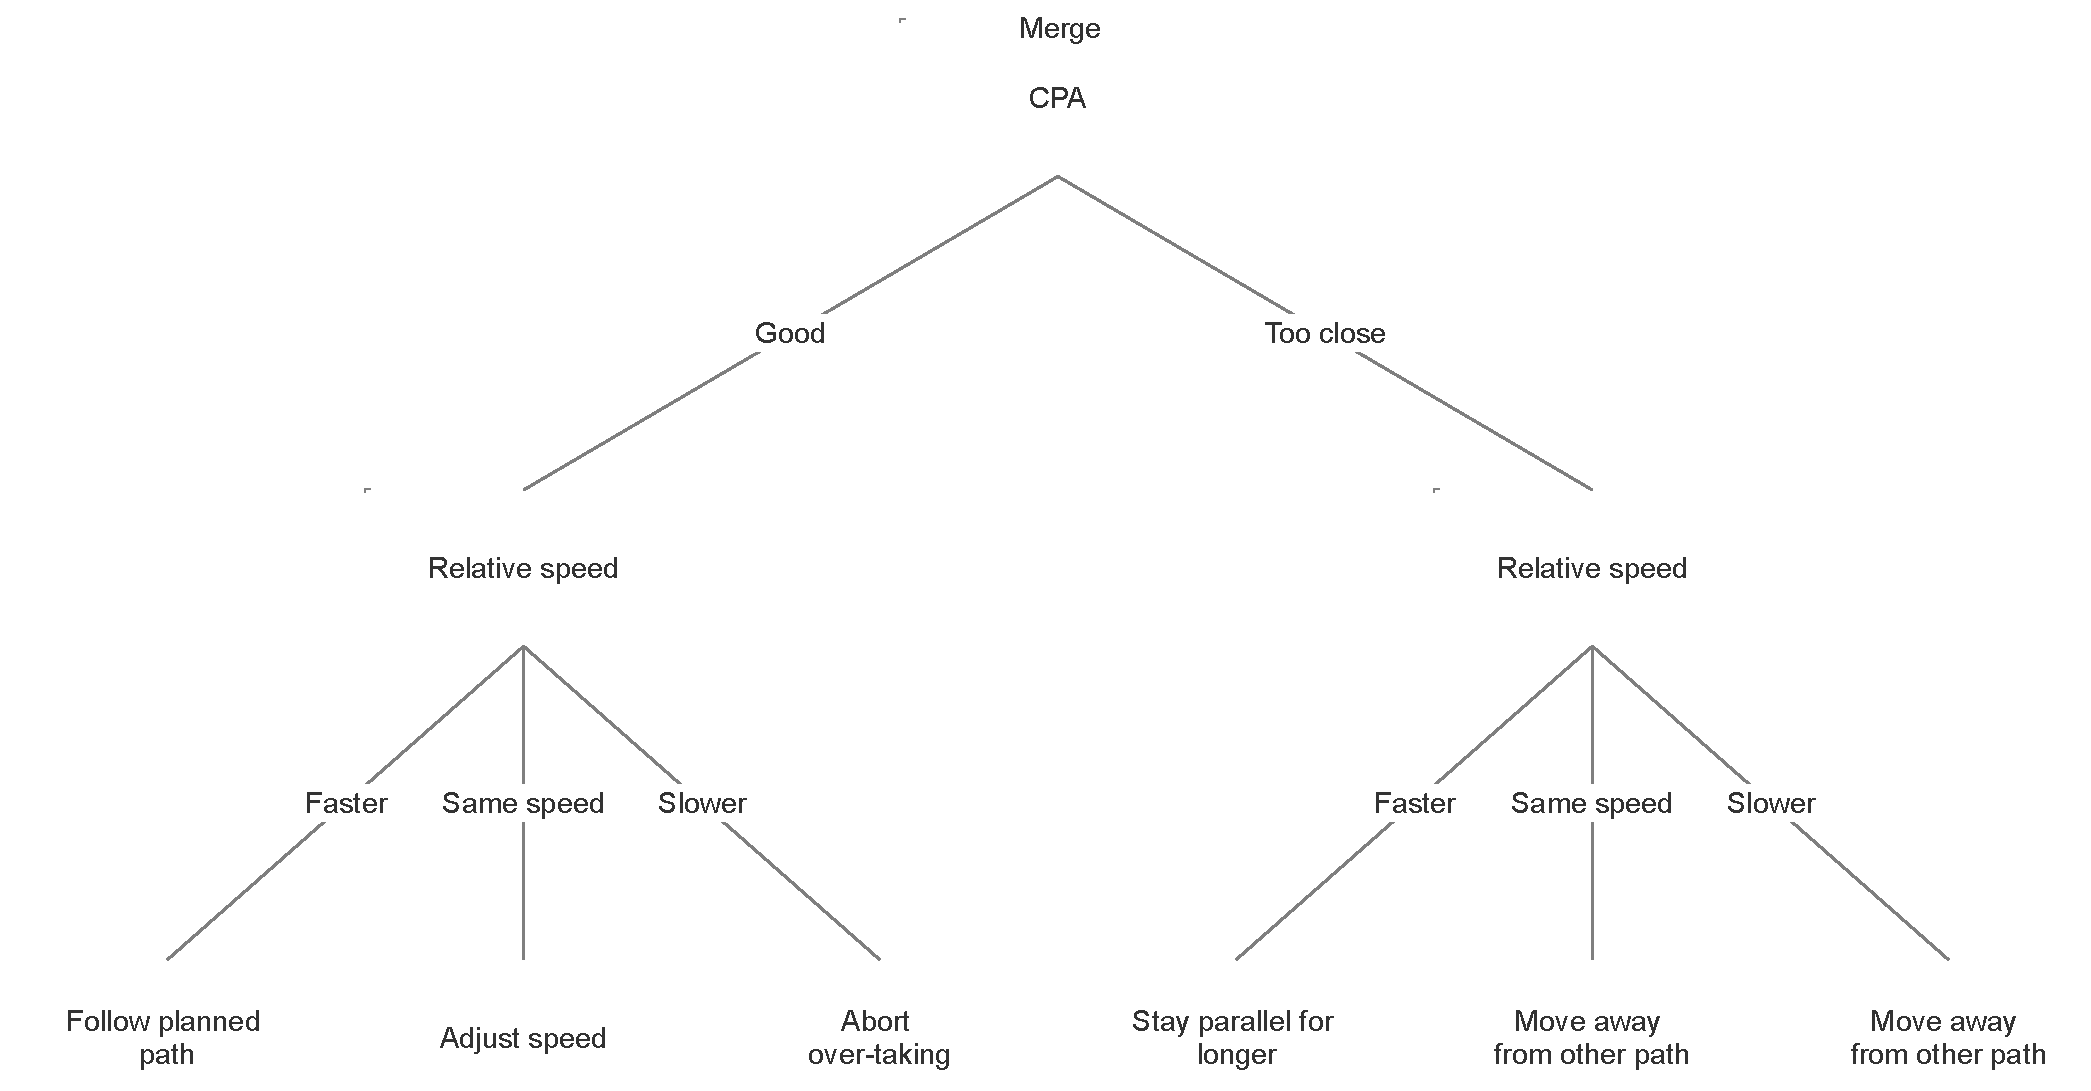
\includegraphics[width=.95\textwidth]{Merge_decision_tree.png}
	\caption{Decision tree when merging}
	\label{fig:Merge_decision_tree}
\end{figure}


\begin{figure}[hp]
	\centering
	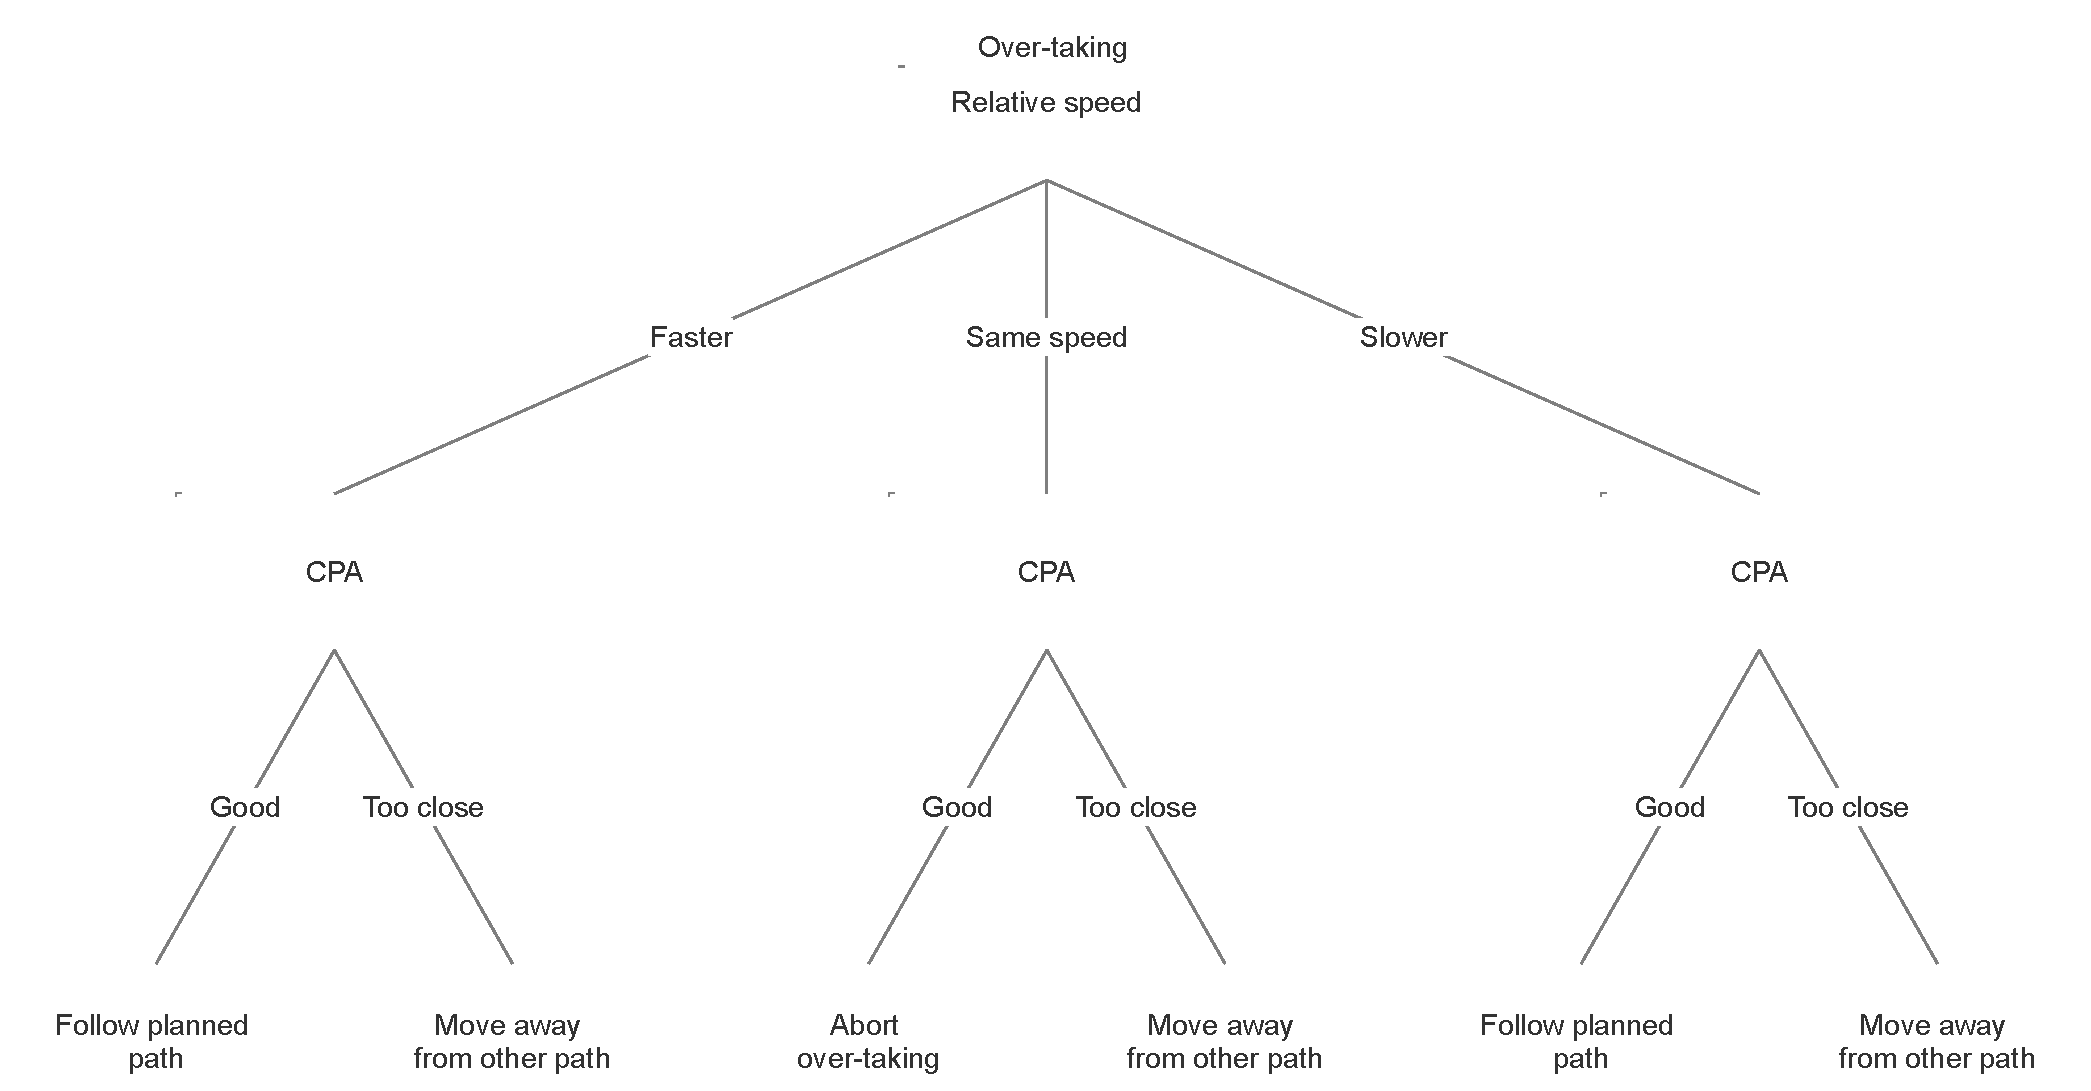
\includegraphics[width=.9\textwidth]{Over-taking_decision_tree.png}
	\caption{Decision tree when over-taking}
	\label{fig:Over-taking_decision_tree}
\end{figure}


\begin{figure}[hp]
	\centering
	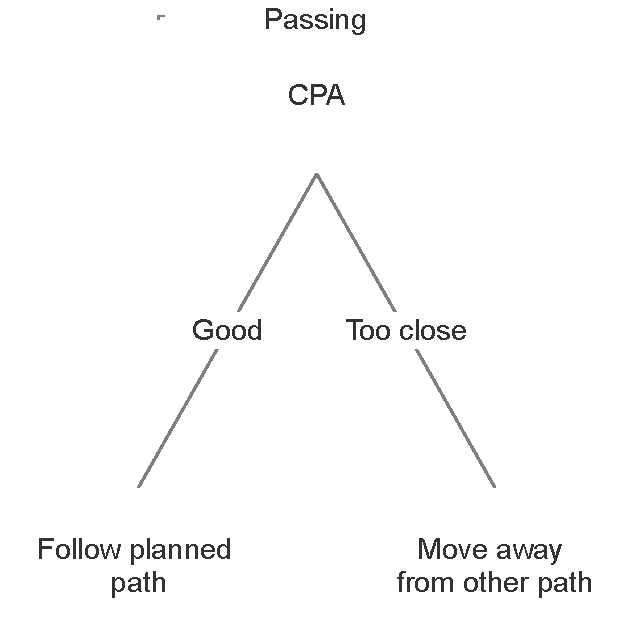
\includegraphics[width=0.2\textwidth]{Passing_decision_tree.png}
	\caption{Decision tree when passing}
	\label{fig:Passing_decision_tree}
\end{figure}

\begin{figure}[hp]
	\centering
	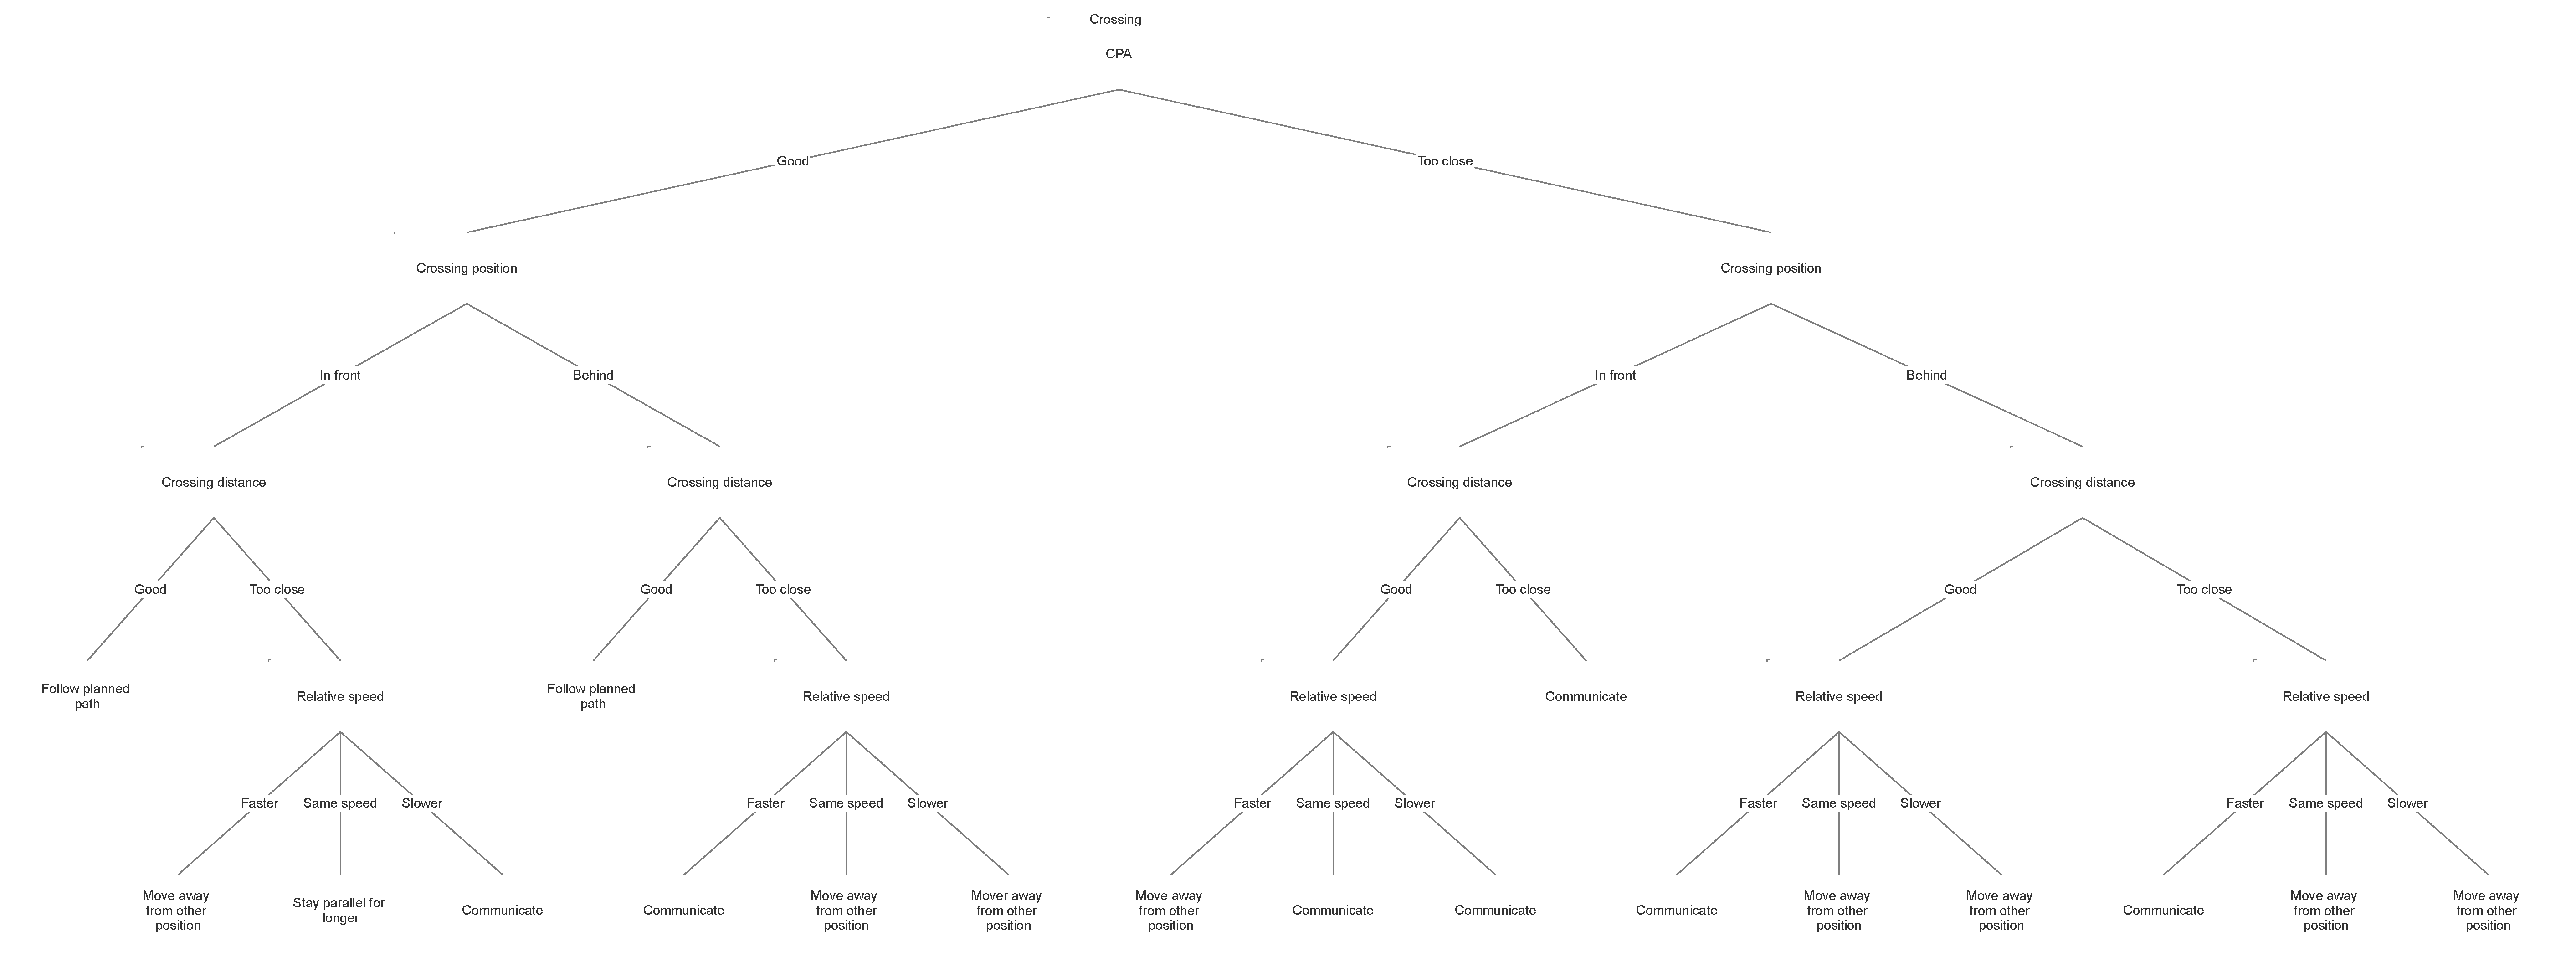
\includegraphics[width=.9\textheight, angle =90 ]{Crossing_decision_tree.png}
	\caption{Decision tree when crossing}
	\label{fig:Crossing_decision_tree}
\end{figure}
	\section{Reported accidents}
\label{sec:accidents}
As mentioned in the introduction is there a desire from the scientific community to do research into the topic of modeling complex systems to improve safety. But the research becomes more relevant if there is a practical application. The clearest case for non-sufficient safety measures is of an accident. Accidents have often been incentives to adapt rules. For example the leading international treaty for safety of life at sea (\ac{SOLAS}) has been adopted in response to the Titanic disaster. But despite new rules, still occur. Below some accidents are discussed and what caused them to happen.

\subsection{Titanic}
The Titanic disaster on 15th April 1912, is on of the most famous accidents in history, an illustation of the collision is shown in figure \ref{fig:Accident-Titanic}. Many things went wrong, which led to the death of more than 1500 people. It is known that the crew ignored warnings for ice packs and ice bergs in the area, as the Titanic did not reduce her speed. When the accident occurred, the ship was sailing almost at top speed, as the captain did not believe the ice was a serious risk to this ship. Thereby did the last minute manoeuvrer to avoid collision fail, causing more damage than a head-on collision. And after the accidents were the distress signals not received by the nearest ship, as the radio operator was off duty and they did not respond to the flares. New regulations and technologies, mitigate the risk of this happening again. But still the human factor led to many accidents.

\begin{figure}[H]
	\centering
	\includegraphics[width=.7\textwidth]{Titanic-accident.png}
	\caption{Illutstration map of approximate collision location}
	\label{fig:Accident-Titanic}
\end{figure}

\newpage
\subsection{Al Oraiq and MV Flinterstar}
During the night between 5 and 6 October 2015 on the Northsea near Zeebrugge, a collision occurred between the LNG tanker Al Oraiq, sailing under the Marshall Islands flag, and the Flinterstar cargo ship, sailing under the Dutch flag. The Flinterstar sank almost immediately as a result of the collision, an illustration of the accident is shown in Figure \ref{fig:Accident-Flinterstar-Al-Oraiq}. The captain of the Flinterstar was badly injured in the incident but the other ten people on board and the pilot were rescued out of the water unharmed.

\begin{figure}[H]
	\centering
	\includegraphics[width=.7\textwidth]{Flinterstar-Al-Oraiq-accident.png}
	\caption{Illutstration map of approximate collision location}
	\label{fig:Accident-Flinterstar-Al-Oraiq}
\end{figure}

The collision occurred because the bridge team on board of the Al Oraiq wrongly assessed the traffic situation, vessel's speed and distance from the S3 buoy, prior to contacting the nearby vessel Thorco Challenger. After informing the Thorco Challenger, did they pass on starboard side. On board of Al Oraiq were coastal pilots witch did not receive feedback from the watch keeping team, nor was there feedback from other vessels via \ac{VHF} radio. The communication which went via VHF radio was mostly in dutch, the officer on duty at Al Oraiq did not request the Coastal pilots to translate. Also did the bridge watch team not asses the situation properly, leading to very little situation awareness.
On board of the Flinterstar there was insufficient attention for watch keeping duties. As several VHF radio communications between Traffic Centre Zeebrugge and other participants within the area monitored by Traffic Centre Zeebrugge, concerning or involving the presence of an inbound LNG carrier were missed by the Pilot and the bridge watch keeping team on board the Flinterstar.
The pilots on board of Al Oraiq did not attempt to work together. Thereby making decisions without consulting the crew, such as overtaking other vessels. Thus the coastal pilot did not act consistent with international understanding, where a pilot is an advisor to the ship's master. Which means mutual understanding for the functions and duties of each other, based upon effective communication and information exchange. 
The sea pilot on board of the Flinterstar got engaged in a casual conversation with the officer of the watch, drawing his attention away from monitoring the traffic situation. The Sea Pilot was advising the officer of the watch from what appeared to be routine. \cite{Backer2015}

\newpage
\subsection{USS Fitzgerald and ACX Crystal}
A more recent well known collision was between the USS Fitzgerald and ACX Crystal on 17th June 2017. The US destroyer hit the larger Philippines container vessel resulting in the death of 7 US Sailors. An illustration of the accident is shown in figure \ref{fig:Accident-USS-Fitzgerald-Crystal}. According to the accident report did failures occurred on the part of leadership and watch-standers. There were failures in planning for safety, adhere basic navigational practice, execute basic watch standing practice, proper use of available navigation tools and wrong responses.

\begin{figure}[H]
	\centering
	\includegraphics[width=.7\textwidth]{USS-Fitzgerald-Crystal-crash.png}
	\caption{Illutstration map of approximate collision location}
	\label{fig:Accident-USS-Fitzgerald-Crystal}
\end{figure}

In accordance with international rules the USS Fitzgerald was obligated to manoeuvrer to remain clear from the other crossing ships. The officer of the deck responsible for navigation and other crew discussed whether to take action but choose not to, till it was too late. While other crew members also failed to provide more situational awareness and input to the officer of the deck. Did the officer of the deck, exhibit poor seamanship by failing to manoeuvrer as required, failing to sound the danger signal and failing to attempt to contact CRYSTAL on Bridge to Bridge radio. In addition, the Officer of the Deck did not call the Commanding Officer as appropriate and prescribed by Navy procedures to allow him to exercise more senior oversight and judgment of the situation. This was prescribed to an unsatisfactory level of knowledge of the international rulles of the nautical road by USS Fitzgerald officers. Thereby were watch team members not familiar with basic radar fundamentals, impeding effective use. Thereby were key supervisors not aware of existing traffic seperation schemes and the expected flow of traffic, as the approved navigation track did not account, nor follow the Vessel Traffic Separation Scheme. Secondary was the automated identification system not used properly. \cite{USSNavy2017}

\newpage
\subsection{USS John S McCain and Alnic MC}
Even more recent is the collision between the USS John S McCain and Alnic MC on 21st August 2017. The US Destroyer hit the Liberia flagged oil and chemical tanker. Resulting in the death of 10  US Sailors. An illustration of the accident is shown in figure \ref{fig:Accident-USS-John-S-McCain-Alnic}. According to the accident report did the US Navy identify the following causes for the collision: Loss of situational awareness in response to mistakes in the operatoin of the USS John S McCain's steering and propulsion system, while in the presence of a high desnity of maritime traffic. Failure to follow the international nautical rules of the road, which govern the manoeuvring of vessels when risk of collision is present. Watchstanders operating the John S McCain's steering and propulsion systems had insufficient proficiency and knowledge of the system. 

\begin{figure}[H]
	\centering
	\includegraphics[width=.7\textwidth]{USS-John-S-McCain-Alnic-accident.png}
	\caption{Illutstration map of approximate collision location}
	\label{fig:Accident-USS-John-S-McCain-Alnic}
\end{figure}

Leading up to the accident did the commanding officer notice that the helmsman had difficulties maintaining course, while also adjusting the throttles for speed control. In response, he ordered the watch team to divide the duties of steering and throttles, maintaining course control with the Helmsman while shifting speed control to another watchstander. This unplanned shift caused confusion in the watch team, which led to wrong transfers of control, where crew was not aware of. 
Watchstanders failed to recognize this configuration. The steering control transfer caused the rudder to go amidships (centerline). Since the Helmsman had been steering less than 4 degrees of right rudder to maintain course before the transfer, the amidships rudder deviated the ship’s course to the left. Additionally, when the Helmsman reported loss of steering, the Commanding Officer slowed the ship to 10 knots and eventually to 5 knots. Due to the wrong transfer did only one shaft slow down, causing an un-commanded turn to the left (port). The commanding officer and others on the ship's bridge lost situational awareness. They did not understand the forces acting on the ship, nor did the understand the Alnic's course and speed relative to USS John S McCain. Three minutes after the reported loss of steering, was it regained, but already too late to avoid collision. No signals of warning were send by neither ship, which are required by international rules of the nautical road. Nor was there an attempt to make contact trough the \ac{VHF} bridge-to-bridge communication.
Many of the decisions made that led to the accident were the result of poor judgemenet and decision making of the commanding officer. That said, no single person bears full responsibility for this incident. The crew was unprepared for the situation in which they found themselves through a lack of preparation, ineffective command and control. Deficiencies in training and preparations for navigation were at the base of this. \cite{USSNavy2017}
	\chapter{Experiment questionnaire}
\label{app:experiment-forms}
\begin{itemize}
	\item Toestemmings verklaring formulier
	\item

\end{itemize}

\end{appendices}


\backmatter

\part{TEMPORARY: Old text}
\chapter*{Manoeuvring capability}
Ship manoeuvring is the ability to keep course, change course, keep track and change speed. Minimal requirements are given by \ac{IMO} standard. However, shipowners may introduce additional requirements. 
Ship manoeuvrability is described by the following characteristics: 
\begin{itemize}
	\item Initial turning ability (start turning)
	\item Sustained turning ability (keep turning)
	\item Yaw checking ability (stop turning motion)
	\item Stopping ability (in rather short distance and time)
	\item Yaw stability (ability to move straight ahead)
\end{itemize}
During sea-trials these capabilities can be determined. However this project will aim at predicting manoeuvrability while using limited input. Thereby is there a difference between the maximum limits and what a ship is likely to do. This will eventually lead to the possible movements of the vessel.

\section*{IMO standard}
The manoeuvrability of a ship is considered satisfactory is the following criteria are complied:
\begin{enumerate}
	\item \emph{Turning ability}. The advance should not exceed 4.5 ship lengths (L) and the tactical diameter should not exceed 5 ship lengths in the turning circle manoeuvre.
	\item \emph{Initial turning ability}. With the application of 10\degree rudder angle to port or starboard, the ship should not have traveled more than 2.5 ship lengths by the time the heading has changed by 10\degree from the original heading. 
	\item \emph{Yaw-checking and course-keeping abilities}. 
	\begin{enumerate}
		\item The value of the first overshoot angle in the 10\degree/10\degree zig-zag test should not exceed: 
		\begin{enumerate}
			\item 10\degree if L/V is less than 10 seconds
			\item 20\degree if L/V is 30 seconds or more
			\item (5 + 1/2(L/V)) degrees if L/V is between 10 and 30 seconds
		\end{enumerate}
		where L and V are expressed in m and m/s, respectively.
		\item The value of the second overshoot angle in the 10\degree/10\degree zig-zag test should not exceed:
		\begin{enumerate}
			\item 25\degree if L/V is less than 10 seconds
			\item 40\degree if L/V is 30 seconds or more
			\item (117.5 + 0.75(L/V)) degrees if L/V is between 10 and 30 seconds
		\end{enumerate}
		\item The value of the first overshoot angle in the 20\degree/20\degree zig-zag test should not exceed 25\degree. 
	\end{enumerate}
	\item \emph{Stopping ability}. The track reach in the full astern stopping test should not exceed 15 ship lengths. However, this value may be modified by the Administration where ships of large displacement make this criterion impracticable, but should in no case exceed	20 ship lengths. 
\end{enumerate}

\section*{Limits}
These standards give guidance during seatrials, but won't help much 
What are maximum values for manoeuvring capability. Based on trial run are values found for Nomoto (other theories?)

Wat is constant? Versnelling/vertraging of de afgeleide daarvan

Clarke, D., Gedling, P. and Hine, G. (1983). The application of manoeuvring criteria in hull design using linear theory. The Naval Architect, pp. 45–68

\section*{Desired capability}
What are normal movements for a ship of a specific size

\section*{Expected route}
Ship will most likely keep sailing straight and on same speed
\todo{describe formula to determine crossingpoint of line}
\todo{CPA calculation}

\section*{Input}
Nomoto, more detailed is Norrbin equation

\subsection*{Detailed capability}
Key equipment for the manoeuvrability are rudders, fixed fins, jet thrusters, propellers, ducts and waterjets. However it is not practical to determine this for every ship which is nearby. Therefore a more statistical approach is taken using comparable ships.






\subsection*{Prediction with limited data}
Own vessel input comes from sea-trial, other vessels based on received information via AIS.
DWT, L, B, speed, etc.


\chapter{Filter situation}
Input from static objects shown on the map

\section{Traffic separation schemes}
input from local authorities

\section{Navigational aids}
map/radar/etc.

\section{Accepted probabilities}
Which probabilities can be ignored to speed-up calculation

\section{Other filters}
Significant wave height/ weather/ windspeed


\chapter{Development of testing environment}
A tool is developed in which can be tested how well decision model works.

\section{Basic design}
To test the different scenarios a tool will be build. This tool will be able to simulate the scenarios to get more insight why decisions are made. Full scale testing will cost much more money, time and effort, as it is harder to control. Small scale testing will introduce many unknown factors. Therefore is chosen to build an application in which models can be tested.
The development will be based on the principles of the Agile Manifesto, as this has proven to result in effective software. This means there will be a start with a basic tool, which will continuously be improved. Changes in requirements might appear trough out the whole process, to deliver a better tool. Thereby must be kept in mind that working software is the primary measure of progress. This is only possible when the software is sustainable and thus easy to maintain and improve, which is only possible with a good design. Keeping it simple will be key in this process. Thereby reflective moments are needed to check if the chosen path is the right one, or if the direction should be adapted. \cite{Agile2001}

\subsection{Requirements}
The first step is to set the goals or requirements of the software. This doesn't mean it is a full description of the software, but features it should at least have to be able to answer the research questions.
The most important requirement is that ships within the simulation behave similarly to ships in reality. This does not necessarily mean that all hydromechanics should be known. But ships should have similar ways of turning and changing speed. This can be based on sea-trials and done using a mapping from current speed, current rotation, rudder angle and throttle to future speed and turning speed.
The second requirement should be that it is flexible, in a way that different scenarios can be added and tested easily. Thereby changing ship characteristics, shared information and other inputs.
Thirdly, it must be possible to show the register of possible decisions for the different vessels. To be able to validate this with seafarers. Meaning it will be a white box model.

\subsection{User stories}
The next step is to define users stories from the requirements. User stories are in a form: \emph{"As a [user] I want [action] so that [result]"}. Extending them with an acceptance criteria this will result in the features which should be implemented.

Within this application there will be different roles. For which these user stories can be used. These can be split between users and objects. Below these are described:
\begin{itemize}
	\item \emph{Operator}. The person who set-up the simulation and fills in the different properties for the ships and specific scenario.
	\item \emph{Viewer}. Someone who uses the application to view a specific scenario. Thereby trying to answer the research questions.
	\item \emph{Ship}. Object in the map which is used by the simulation. But to work correctly it also had needs for information.
\end{itemize}

Some examples of those user stories are given below. All users stories can be found in appendix XXX.\todo{add user stories to appendix}. 

\begin{itemize}
	\item As an operator, I want to add vessels to the map, by selecting them in a list, so that they become part of the simulation. \\
	Acceptance criteria: Ship visualized and other ships start receiving information.
	\item As a viewer, I want to to be able to get the belief state, intention and next action of a ship, so that I can verify if it is what I expected it to be. \\
	Acceptance criteria: Belief state, intention and next action are shown.
	\item As a ship, I want to be able to predict the path of other vessels, so that I can make my decisions based on this. \\
	Acceptance criteria: correctly updated belief state about other vessels.
\end{itemize}

\subsection{User interactions}
What should be done in the different modules

\subsection{Minimum viable product}
Considering the above mentioned requirements and user stories. Not everything is within the scope, and thus shouldn't be developed and implemented. Examples of possible features which are not implemented are: ... 
There must also be considered that several assumptions are made to create a system which works in a practical manner, as not al input data is available or calculations might be very hard and slow down the simulation too much. The assumptions made are: ...

Thereby should be kept in mind that the acceptance criteria for the application is: The ability to insert a model for decision making for a ship, which depends on information collected from other ships closeby, its own ship characteristics and the environment it acts in.
\todo{Extent the acceptance criteria for the full application}

\section{Manoeuvring capability model}
Estimation of relation between throttle, loss of speed while turning. Thus a mapping from current speed, current rotation, rudder angle and throttle to future speed and turning speed

\section{Probability index}
what should the polygons show

\section{Radio}
The area in which situations are tested are not larger than the radius of an VHF radio (about 20 NM - IMO regulations)

\url{http://solasv.mcga.gov.uk/m_notice/mgn/mgn324.pdf} - p8

Therefore a ra

\section{Controller}
Based on the waypoints there is a simple controller to adjust the rudder angle. This controller steers based on the relative angle between the waypoint and the current position. This is done in the \emph{adjustRudder} function. The distance and relative angle is calculated, this is used in a simple decision tree to decide on the rudder angle, which is similar to a so-called "proportional controller". For this simulation it will give enough accuracy. For a better result, a "PID-controller" could be implemented:

\begin{table}[H]
	\centering
	\begin{tabular}{l|l}
		\toprule
		Relative angle (\degree) & Rudder angle (\degree) \\
		\midrule
		25-180 & 35\\
		10-25 & 25\\
		0-10 & Relative angle $*$ 8/10 \\
		\bottomrule
	\end{tabular}
	
	\captionof{table}{Rudder angle based on relative angle}
	\label{tab:Rudder-angle}
\end{table}

\section{Estimation of characteristics}
Deadweight to displacement for example

\section{Application design}
Building and verification including description of the architecture. Model-view-controller architecture, for easy modification as there are less dependencies between modules.

\subsection{Design patterns}
Push-pull listener

\subsection{Model and classes}
Use list from excel, make simple drawing how they link an talk to each other. Based on model-view-controller.

\subsection{Methods}
Full list in appendix XXX, describe important methods and how design patterns are used. Push-pull for example

\subsection{User interface}
Some screenshots of the application with a description what can be controlled and seen. Implementation of models is not relevant yet.

\addcontentsline{toc}{chapter}{Bibliography}
\bibliography{include/library}




\end{document}

